\documentclass[12pt]{article}

% Packages

\usepackage{caption}
\usepackage{fbb} % for addition of Bembo font
\usepackage[T1]{fontenc}
\usepackage{graphicx}
\usepackage[hidelinks]{hyperref}
\usepackage[utf8]{inputenc}
\usepackage{lastpage} % count pages
\usepackage{lineno} %for line numbering
\usepackage{natbib}
\usepackage{setspace} %for line spacing
\usepackage{titlesec}
\titlelabel{\thetitle\hspace{0.5cm}|\quad}
\renewcommand\tablename{TABLE}
\renewcommand\figurename{FIGURE}
\captionsetup[table]{labelsep=quad}
\captionsetup[figure]{labelsep=quad}

% Margin setup

\RequirePackage{geometry}
\geometry{
	paper=a4paper,
	inner=3.0cm,
	outer=3.0cm,
	top=2.75cm,
	bottom=2.5cm,
	headheight=20pt, 
	headsep=.25in,
	includehead,
	includefoot
}

% For fixed table column widths

\usepackage{array}
\newcolumntype{L}{>{\centering\arraybackslash}m{4cm}} %both for allowing text-wrap in tables
\newcolumntype{B}{>{\centering\arraybackslash}m{3cm}}

\newcommand{\bbletterm}{{\textsf{m}\hspace*{-1.0ex}%
  \rule{0.15ex}{1.3ex}\hspace*{1.0ex}}}

\begin{document}

\linenumbers
\fontsize{12pt}{12pt}\selectfont

\section*{Abstract}

\noindent 1. For many vertebrates, urban environments are characterised by frequent environmental stressors. Coping with such stressors can demand that urban individuals activate energetically costly physiological pathways more regularly than rural-living conspecifics. However, urban environments also commonly demand appreciable expenditure toward thermoregulation, owing to their often extreme climatic variation. To date, whether and how vertebrates can balance expenditure toward both the physiological stress response and thermoregulation, and thus persist in an urbanising world, remains an unanswered and urgent question among ecologists. 
\vspace{\baselineskip}

\noindent 2. We tested whether changes in body surface temperature (T\textsubscript{s}) and peripheral heat loss (q\textsubscript{Tot}) that accompany the stress response: (1) endow urban individuals with an enhanced capacity to conserve heat in the cold, and dissipate heat in the warmth relative to rural conspecifics, and (2) meet an essential first criterion for evolutionary responses to selection (variability among, and consistency within individuals). 
\vspace{\baselineskip}

\noindent 3. Using the black-capped chickadee (n = 19) as a model species, we show that neither rapid nor chronic changes in T\textsubscript{s} and q\textsubscript{Tot} following stress exposure differed between urban- and rural-origin individuals (n\textsubscript{urban} = 9; n\textsubscript{rural} = 10). Nevertheless, we do find that stress-induced changes in T\textsubscript{s} and q\textsubscript{Tot} are highly repeatable across chronic time periods (R\textsubscript{Ts} = 0.61; R\textsubscript{qTot} = 0.67) and display signatures of stabilising or directional selection (i.e. reduced variability and increase repeatability relative to controls). 
\vspace{\baselineskip}

\noindent 4. Our findings suggest that, although urban individuals appear no more able to balance expenditure toward thermoregulation and the stress response than rural conspecifics, the capacity to do so may still be subject to selection in chickadees.
\vspace{\baselineskip}
\vspace{\baselineskip}

\par\noindent \textbf{Keywords}; Flexibility, Stress, Thermoregulation, Repeatability

\clearpage

\fontsize{12pt}{24pt}\selectfont
\section{INTRODUCTION}
\vspace{0.5cm}

\noindent Over the past 70 years, the global human population has increased by approximately 350\% (or approximately 5.1 billion; \citealt{un_2019}). Unlike in previous centuries, the majority of individuals (nearly 54\%) now reside in urban environments, and global trends strongly suggest that urban living will increasingly become the norm (reviewed in \citealt{lerch_2017}). Consequently, land area designated for urban utility is expanding at unprecedented rates and will probably continue to do so over the coming decades \citep{angel_2011}. Such expansion cannot, however, occur in a vacuum, and has thus contributed to the widespread reduction in habitat availability and quality for many species (\citealt{grimm_2008,seto_2012,freeman_2019}; lay literature: \citealt{thomas_2017}). For this reason, understanding whether these species can adapt and persist within modern city-scapes has become a growing priority among modern ecologists and conservationists (e.g. \citealt{birnie_2016,ouyang_2018}). \vspace{1cm}

\noindent Habitat loss or degradation are not the only challenges faced by species in urban environments. Indeed, urban environments regularly present acute challenges, including noise, frequent human interaction, vehicle traffic, and in some cases, elevated depredation and inter- and intra-specific competition (\citealt{johnson_2012,hernandez_2014,newsome_2015,vincze_2017}; reviewed in \citealt{lowry_2013}). Coping with these acute challenges can demand that individuals within urban environments activate self-preserving physiological responses (i.e. fight-or-flight responses) more regularly than rural-living conspecifics (\citealt{bonier_2012,watson_2017}; albeit, often with reduced intensity; \citealt{partecke_2006,french_2008}; but see \citealt{fokidis_2009}). While such demands need not inherently translate to a loss of fitness among urban individuals, laboratory studies suggest that their daily metabolic costs are probably raised owing to increased allostatic load \citep{depke_2008,jimeno_2017}. In turn, these elevated metabolic demands may enhance susceptibility to wear and tear when resources are restricted or are required to be allocated elsewhere \citep{romero_2009,breuner_2019}. \vspace{1cm}

\noindent Beyond urban development, many of today's species face additional and indirect threats associated with a growing human population. Effects of anthropogenic climate change on species distribution and trait expression, for example, have now been argued for nearly all taxa (e.g. \citealt{barton_2016,mainwaring_2017,pacifici_2017,wan_2018}), and concerns over the ability of species to adjust to rising and increasingly variable ambient temperatures \citep{vasseur_2014} have been well articulated (e.g. \citealt{duputie_2015,radchuk_2019}). In endotherms, increases in both maximal ambient temperature and variability of ambient temperatures can bear notable thermoregulatory costs \citep{pendlebury_2004,duplessis_2012,smit_2018}, with those associated with the former being particularly severe in urban environments \citep{arnfield_2003}. These costs, coupled with expected increases in susceptibility of wear and tear, beg important questions of whether and how endotherms may cope with increasingly urbanised environments in the face of a rapidly changing climate (discussed in \citealt{pautasso_2012,argueso_2015, brans_2017}). \vspace{1cm}

\noindent To date, several empirical studies have shown that endotherms may adjust their superficial blood-flow, and thus, their body surface temperatures (henceforth, "T\textsubscript{s}") when exposed to stressors (e.g. \citealt{blair_1959,yokoi_1966,nord_2019b,winder_2020}). In some species, these changes in T\textsubscript{s} appear to endow individuals with greater heat conservation in the cold, and greater heat dissipation in the warmth, thus reducing their demands for costly thermogenesis or evaporative cooling respectively (\citealt{jerem_2018,robertson_2020a,winder_2020}). In this way, total energetic expenditure may be balanced in challenging environments by allocating energy toward more immediate and higher-cost threats (e.g. the perceived stressors) and away from less immediate and lower-cost threats (e.g. thermal challenges; \citealt{jerem_2018,robertson_2020a}). In urban environments, where individuals regularly contend with both physical and thermal challenges, such flexibility of T\textsubscript{s} and peripheral heat loss (here, non-evaporative heat-loss; henceforth, "q\textsubscript{Tot}") could be particularly advantageous, with those capable of enhanced flexibility (particularly during stress exposures) being better able to balance energy expenditure and, therefore, being favoured by selection \citep{parsons_2005}. Nevertheless, the potential for selection to act on flexibility of T\textsubscript{s} and q\textsubscript{Tot} in response to stressors requires that these traits are both variable among individuals, and consistent within individuals (i.e. "repeatable"; reviewed in \citealt{boake_1989,wolak_2012}). Over the past two decades, numerous studies have reported moderate to high degrees of repeatability among traits associated with the stress response and whole-animal metabolism (\citealt{nespolo_2007,rensel_2011,muller_2018,boratynski_2019}; but see \citealt{ouyang_2011}). While these finding strongly suggest that stress-induced changes in T\textsubscript{s} and q\textsubscript{Tot} are also likely to be repeatable in endotherms, the degree of this repeatability remains largely unclear (but see \citealt{careau_2012}). \vspace{1cm}

\noindent Using the black-capped chickadee (\textit{Poecile atricapillus}; henceforth "chickadees") as a model species, we tested whether flexibility of both T\textsubscript{s} and q\textsubscript{Tot} during stress exposure: (1) meet critical first criteria for responsiveness to selection, and (2) offer opportunities for endotherms to cope with the increased allostatic and thermoregulatory costs of an urbanising environment. More specifically, we hypothesised that stress-induced changes in both T\textsubscript{s} and q\textsubscript{Tot}: (1) are variable among, and consistent within individuals, (2) provide evidence of current or past selection, and (3) differ between individuals captured from urban and rural environments. Accordingly, we first predicted that stress-induced changes in both T\textsubscript{s} and q\textsubscript{Tot} would be repeatable among individuals. Because thermal responses to stress exposure can be acute (e.g. minutes to hours: \citealt{jerem_2015,andreasson_2020b,winder_2020}) or chronic (e.g. days: \citealt{bittencourt_2015,herborn_2018}), and responses across each time-period may provide energetic benefits by enhancing heat dissipation or relaxing costs of thermogenesis (\citealt{jerem_2018,herborn_2018,winder_2020}), we predicted that both acute and chronic changes in T\textsubscript{s} and q\textsubscript{Tot} accompanying the stress response would be repeatable among individuals in our sample population. Next, because traits subject to previous or current selection (here, directional or stabilising) are thought to display lower variability and higher repeatability than those that are selectively neutral (e.g. \citealt{gibson_1974,lande_1983,boake_1989,vanhomrigh_2007}; but see \citealt{kotiaho_2001}), we predicted that both T\textsubscript{s} and q\textsubscript{Tot} of chickadees would be less variable and more repeatable during stress exposure treatments than during control treatments, after controlling for predictable environmental effects on heat loss (e.g. ambient temperature and relative solar radiation). Finally, because the combined energetic costs of stress exposure and thermoregulation are expected to be higher in urban environments when compared with rural environments (i.e. in the absence of phenotypic differences between urban and rural individuals; discussed above), we predicted that the magnitude of both acute and chronic changes in T\textsubscript{s} and q\textsubscript{Tot} that accompany stress exposures would be larger among urban-origin individuals than rural-origin individuals. \vspace{1cm}

\noindent To test our predictions, we exposed chickadees captured from urban and rural environments to both repeated stressors and control conditions across an ambient temperature gradient while monitoring rapid and long-term changes in T\textsubscript{s} and q\textsubscript{Tot} by infra-red thermography. In small birds, surface tissues at the periorbital region (henceforth "eye region") are thought to play a critical role in environmental heat exchange (e.g. \citealt{hill_1980,powers_2015}) and both temperature of, and heat loss from this region have previously been shown to respond to stress exposure (e.g. \citealt{jerem_2015,ikkatai_2015,herborn_2018,robertson_2020a}). We, therefore, chose to use temperature of, and heat loss from, the eye region as our indicators of T\textsubscript{s} and q\textsubscript{Tot} in this study. \vspace{1cm}

\noindent The capacity of vertebrates to cope with the combined pressures of urbanisation and anthropogenic climate change has been questioned many times \citep{pautasso_2012,argueso_2015,brans_2017}. The proximate physiological mechanisms by which vertebrates (here, endotherms) may do so, however, are seldom explored. Ours study, therefore, represents a critical step forward in how ecologists might test the capacity of vertebrates to adapt an increasingly human-modified world. \vspace{0.5cm}

\section{MATERIALS AND METHODS}
\vspace{0.5cm}

\noindent All methods used for animal capture, sampling, and experimental treatment were approved by the Trent University Animal Care Committee (AUP \# 24614) and Environment and Climate Change Canada (permit \# 10756E).\vspace{0.5cm}

\subsection{Capture, transport, and housing of experimental animals}
\vspace{0.5cm}

\noindent Chickadees (n = 20; n = 10 females, n = 10 males) used for this experiment were captured within a 100 km\textsuperscript{2} region of south-western Ontario, Canada, between the months of March and April in 2018. To minimise the possibility of kinship between individuals within our sample population, capture efforts were divided across six distinct locations (three urban and three rural), each separated by a minimum distance of 15 km. Urban capture locations included the downtown regions of the cities of Brantford (43.1345$^{\circ}$N, 80.3439$^{\circ}$W), Cambridge (43.3789$^{\circ}$N, 80.3525$^{\circ}$W), and Guelph (43.3300$^{\circ}$N, 80.1500$^{\circ}$W), while rural capture locations included the townships of Corwhin (43.5090$^{\circ}$N, 80.0899$^{\circ}$W), Erin (43.7617$^{\circ}$N, 80.1529$^{\circ}$W), and Cayuga (42.9797$^{\circ}$N, 79.8745$^{\circ}$W)(\hyperref[FigC.1]{SFigure 1}). A difference in the mean degree of urbanisation between urban and rural capture locations was validated using methods similar to Thompson et al (\citeyear{thompson_2018}; see Appendix; \hyperref[FigC.2]{SFigures 2}-\hyperref[FigC.4]{4}). \vspace{1cm}

\noindent All individuals were captured using modified potter traps (dimensions [L $\times$ W $\times$ H] = 90 $\times$ 70 $\times$ 70 cm), baited with sunflower seeds and suet on the day of capture. To further draw individuals to trap locations, we alternately broad-casted chickadee breeding songs and alarm calls from a remote call-box (FoxPro\textsuperscript{TM} Patriot; Lewisville, PA, USA) until at least one individual approached a potter trap by $\leq$ 4 meters. Upon capture, chickadees were blood sampled (approximately 50 $\mu$L) by brachial venipuncture and capillary tube collection, then fitted with one stainless steel, numbered leg ring (size 0) and a unique combination of two, coloured, Darvic leg rings (size 0) for future identification. Each individual was then measured (mass to the nearest 0.1 g using an electronic scale, and, wing cord to the nearest 0.1 mm, left outer tarsus to the nearest 0.1 mm, and head-to-bill to the nearest 0.1 mm using analogue calipers) and secured in a covered flight enclosure (dimensions [L $\times$ W $\times$ H] = 30 $\times$ 30 $\times$ 15 cm) for transportation to our long-term housing facility (Ruthven Park National Historic Site, Cayuga, Ontario; $\leq$ 90 km drive). Blood samples were preserved in a small volume of Queen's Lysis buffer (500 $\mu$L; \citealt{seutin_1991}) for use in genetic sexing (using methods described in \citealt{robertson_2020a}) and were held on ice until storage at 4$^{\circ}$C was possible ($\leq$ 2 hours). \vspace{1cm}

\noindent Upon arrival to our long-term housing facility, chickadees were haphazardly distributed among four, visually isolated flight enclosures (n = 5 per enclosure; dimensions [L $\times$ W $\times$ H] = 1.83 $\times$ 1.22 $\times$ 2.44 m), each equipped with one white cedar tree (\textit{Thuja occidentalis}), two perching branches (raised to approximately 1.50 and 1.80 m above ground) and a raised feeding platform (400 cm\textsuperscript{2}) at which food was provided \textit{ad libitum} through an opaque hinged door for the duration of the experiment (\hyperref[Fig4.1]{Figure 1}). Food provided included sunflower seed, safflower seed, shelled peanuts, boiled egg, apple pieces, house crickets (\textit{Acheta domesticus}), meals worms (\textit{Tenebrio molitor}) and Mazuri (St Louis, MO, USA) Small Bird Maintenance diet. Water was also provided \textit{ad libitum} across our experiment through opaque hinged doors. All individuals were given a minimum of 2 weeks to acclimate to enclosures and social groups prior to onset of experimentation. \vspace{0.5cm}

\subsection{Experimental stress exposure}
\vspace{0.5cm}

\noindent To test repeatability of stress-induced thermal responses within and among individuals, we used a paired experimental design wherein each individual was exposed to both a thirty-day control treatment and a thirty-day stress exposure treatment, with treatments separated by an additional two-day control period (total experimental duration = 62 days). To control for possible effects of treatment order on stress-induced thermal responses, half of our sample population (n = 10 across two flight enclosures) was exposed to control treatments followed by stress-exposure treatments, while the second half of our sample population (n = 10 across two flight enclosures) was concurrently exposed to a reversed treatment order (i.e. stress-exposure treatments followed by control treatments). \vspace{1cm} 

\noindent Each day, individuals within stress exposure treatments were exposed to 5 or 6 experimental stressors, with each being applied for 20 minutes and being separated from previous and subsequent stress exposures by $\geq$ 1 hour (similar to \citealt{rich_2005}). Timing and type of experimental stressors were randomly selected each day to minimise the potential for habituation to each given stressor type. Experimental stressors included the presence of a novel object (a garden gnome), presence of a mock predator (a taxidermically mounted Cooper's hawk; \textit{Accipiter cooperii}), capture and restraint in an opaque fabric bag, presence of a human, covering of a given flight enclosure with an opaque tarp (simulating extreme, inclement weather), and presence of a taxidermically mounted conspecific fixed to the feeding platform of a given flight enclosure (simulating a novel, dominant individual). In a previous study, chickadees exposed to our randomised stressor protocol displayed a significant reduction in feeding rate and mass, and regularly evoked alarm calls (\citealt{robertson_2020b}), providing strong support for protocol efficacy. Endocrine responses to stressor types were not measured to circumvent effects of blood sampling on surface temperature measurements and stress perception among sampled individuals. Individuals exposed to control treatments were left undisturbed in an adjacent flight enclosure and blind to experimenter presence. \vspace{1cm}    

\noindent Because flight enclosures were not auditorily segregated, estimated thermal responses to stress exposure in this study (i.e., the interaction between time or ambient temperature and treatment type) are expected to be conservative. \vspace{0.5cm}

\subsection{Infrared thermography, body surface temperature estimation, and heat transfer estimation}
\vspace{0.5cm}

\noindent We monitored T\textsubscript{s} and q\textsubscript{Tot} of chickadees indirectly using remote infra-red thermography (thermographic camera: FLIR VueProR\textsuperscript{TM}, 13 mm, 226 $\times$ 356 resolution: accuracy = $\pm$ 5\%; image frequency = 1 Hz). Specifically, we captured infrared thermographic images (radiometric JPEGs) of individuals at feeding platforms across the duration of our experiment from weather-proofed camera boxes mounted to the exterior of enclosure walls (0.5 m distance). To minimise temporal bias of thermographic imaging among social groups, we rotated our thermographic camera cardinally clock-wise among flight enclosures each day, with filming durations persisting for approximately one hour per enclosure, and the first flight enclosure to receive thermographic filming being rotated each day. Because leg-ring combinations could not be readily distinguished from thermographic images, we also captured digital video (camera: Action Cam\textsuperscript{TM}, Sony, Toronto, Ontario, CA) of feeding individuals in parallel to themographic images to permit individual identification. All thermographic imaging and digital video used in this study were captured between 08:00h and 16:00h of each day. \vspace{1cm}
  
\noindent Estimation of an object's T\textsubscript{s}, and consequently rate of heat transfer (q\textsubscript{Tot}) by infrared thermography requires that local ambient temperature and relative humidity are known \citep{minkina_2009,tattersall_2016}. We therefore monitored ambient temperature at enclosures subjected to thermographic filming using a ThermoChron iButton\textsuperscript{TM} (Maxim Integrated, DS1922L-F5, San Jose, CA, USA) placed in the shade, at a frequency of 1 reading/5 minutes. Relative humidity readings were collected from a nearby weather station operated by Environment and Climate Change Canada (station identity = Hamilton A, 22 km from the experimental holding location) at the maximum available frequency of 1 reading/hour. \vspace{1cm} 

\noindent To estimate T\textsubscript{s} from infrared thermographic images, we followed methods described elsewhere \citep{robertson_2020a}. Specifically, raw infra-red radiance (kW/m\textsuperscript{2}) values per pixel were manually extracted in R statistical software (version 3.6.1; \citealt{rcore_2019}) then first converted to temperature ($^{\circ}$C) per pixel according to Planck's law, ambient temperature, and humidity estimates at the time of image capture, and equations outlined elsewhere (\citealt{minkina_2009,tattersall_2016}). Emissivity of the eye region of chickadees was assumed to be fixed at 0.95 according to estimates made for integument of Canadian and snow geese (\textit{Branta canadensis} and \textit{Chen caerulescens} respectively; \citealt{best_1981}). Following their estimation, temperature values per pixel were then integrated into FITS matrices using the R package FITSio (version 2.1.0; \citealt{harris_2016}; one matrix per thermographic image), and eye region T\textsubscript{s} values (here, maximum temperature values, as per \citealt{jerem_2015}) were manually extracted from within matrices using the open-sourced software FIJI (\citealt{schindelin_2012}; average size of eye region $\approx$ 230 pixels). To minimise underestimation of T\textsubscript{s} as a consequence of image blurring, only values extracted from individuals that were stationary during image capture were included in our final data \citep{tattersall_2016}. \vspace{1cm}

\noindent To estimate q\textsubscript{Tot} (mW) from T\textsubscript{s} measurements, we followed equations described by \citet{mccafferty_2011} and \citet{nord_2019}. Here, however, values for the kinematic viscosity of air (m\textsuperscript{2}/S; at an assumed atmospheric pressure of 101.325 kPa) and the thermal expansion coefficient of air (1/K) were estimated for each given ambient temperature using the R packages "bigleaf" and "Thermimage" respectively \citep{bigleaf,thermimage}. For this study, q\textsubscript{Tot} was assumed to equal the sum of convective and radiative heat transfer, owing to both the minimal effects of wind-speed in our flight enclosures, and low likelihood of heat transfer between the eye region and any medium other than air during our experiment. Surface area of the eye region was estimated as 0.864 cm\textsuperscript{2} (ovoid with horizontal diameter of 1.1 cm and vertical diameter of 1.0 cm), and contours within the eye region were considered negligible. Final q\textsubscript{Tot} estimates were multiplied by two to represent q\textsubscript{Tot} across both eye regions.\vspace{0.5cm}

\subsection{Statistical analyses}
\vspace{0.5cm}

\noindent All statistical analyses were conducted in R software (version 3.6.1; \citealt{rcore_2019} with each generalised additive mixed-effects model ("GAMM") constructed in the package "brms" (version 2.13.3; \citealt{burkner_2017}). Additionally, all models were run using Markov Chain Monte Carlo (MCMC) sampling, with 4 Markov chains, 10000 chain iterations, and 1000 warm-up iterations to maximise mixing and convergence of Markov chains. Final iterations were thinned by 10 to account for possible autocorrelation between MCMC draws, and models were validated by visually diagnosing residual distributions and trace plots. $\hat{R}$ values for all model parameters fell between 0.99 and 1.01, and the ratio of effective sample sizes to our total sample size were greater than 0.65 for each parameter. Lastly, all figures were produced in R using the package "ggplot2" (version 3.3.2; \citealt{wickham_2016}), and one individual (a female captured in an urban environment) was removed due to an unusually small sample size (n = 19 thermographic images).\vspace{0.5cm}

\subsubsection{Thermal responses to stress exposure among individuals} 
\vspace{0.5cm}

\noindent To first test whether acute and chronic changes in T\textsubscript{s} accompanying the stress responses were repeatable among individuals, we constructed two Bayesian hierarchical GAMMs wherein we estimated both global responses and individual-level responses to stress exposure across acute and chronic time scales. In both models, temperature of the eye region of individuals ($^{\circ}$C; Gaussian distributed) was included as the response variable, and treatment type (i.e. stress exposure or control) and sex were included as linear, population-level predictors to account for the influence of each on eye region temperature measurements. Additionally, flight enclosure identity, date of thermographic image capture, and individual identity were included in each model as group-level intercepts to account for statistical non-independence between measurements collected from the same flight enclosure, day, and individual, and a group-level slope for time of day per flight enclosure orientation (i.e. east facing or west facing) was included to account for differential exposure to solar radiation within east- and west-facing enclosures across time. \vspace{1cm}

\noindent In our model predicting acute thermal responses to stress-exposure, time post stress exposure (seconds), ambient temperature, and time of day (hour) were each included as population level predictors. Because acute, stress-induced changes in T\textsubscript{s} at the eye region are thought to be non-linear \citep{jerem_2015,jerem_2019}, time post-stress exposure was included as a cyclic cubic regression spline with 5 knots fixed at -1200, 0, 1200, 2400, and 3600 seconds to evenly distribute model fitting across each phase of stress exposure (i.e. before, during, and after exposure). Here, a cyclic regression spline was chosen to capture expected returns to baseline T\textsubscript{s} (as reported for blue tits, \textit{Cyanistes caeruleus}; \citealt{jerem_2019}) following 40 minute recovery periods. To permit comparisons between stress exposed and control treatments, we paired enclosures such that time post stress exposure for an enclosure experiencing a control treatment was considered to be equivalent to that of the nearest enclosure experiencing a stress exposure treatment and equivalent cardinal orientation (i.e. west- or east- facing). As such, our comparisons between treatments account for indirect effects of experimental stress exposures on nearby control individuals. \vspace{1cm}

\noindent In endotherms, T\textsubscript{s} is expected to display non-linear relationships with both ambient temperature and time of day owing to peripheral thermoregulatory processes (i.e. cold-induced vasoconstriction and warm-induced vasodilation) and circadian rhythms \citep{richards_1971,cooper_2005} respectively. Ambient temperature and time of day were therefore included as natural cubic and thinplate regression splines respectively, each with 4 knots to minimise risk of model over-fitting. Knots for our ambient temperature spline were evenly spaced by quantiles to uniformly capture trends in eye region temperature at ambient temperatures below, within, and above thermoneutrality for our study species \citep{grossman_1977}. Because we did not have \textit{a priori} assumptions for knot positions for our time of day spline, knot positions were chosen by truncated eigen decomposition \citep{wood_2003}. To control for differential effects of treatment type on T\textsubscript{s} across time \citep{jerem_2015,jerem_2019} and ambient temperature (\citealt{robertson_2020a}), population-level interactions between treatment type and ambient temperature, and treatment type and post stress exposure were also included as model predictors, along with an interaction between treatment type and the tensor product ($\otimes$) between ambient temperature and time post stress exposure to account for the influence of ambient temperature on acute thermal responses to stress exposure at the skin \citep{nord_2019b}. All interaction terms were penalised on the first derivative to minimise the potential for concurvity between interaction terms and main effects. Finally, to estimate differences in acute, stress-induced changes in T\textsubscript{s} among individuals, group-level slopes for time post stress exposure and the interaction between time post-stress exposure and treatment type were included for each individual. Correlations between adjacent T\textsubscript{s} measurements was corrected using a type-I autoregressive (AR1) correlation structure with an estimated rho ($\rho$) of 0.69, and residual error was estimated independently for each treatment type. \vspace{1cm} 

\noindent In our model predicting chronic stress-induced changes in T\textsubscript{s}, group-level predictors remained as described above but with minor adjustments. Specifically, all predictors including time post stress exposure (i.e. as a main effect or interactive effective) were excluded from our model to permit assessment of long-term, but not short-term trends in T\textsubscript{s} according to treatment type. Furthermore, to estimate differences in chronic stress-induced changes in T\textsubscript{s} among individuals, group-level slopes for ambient temperature and the interaction between ambient temperature and treatment type was included per individual. Here, ambient temperature was mean-centered and scaled to 2 times the standard deviation (as per \citealt{araya_2015}) to allow for individual slopes to be estimated with respect to our average environmental conditions. Again, correlations between adjacent T\textsubscript{s} measurements was corrected using an AR1 correlation structure ($\rho$ = 0.69), and residual error was estimated separately per treatment. \vspace{1cm}

\noindent Because rates of peripheral heat transfer (q\textsubscript{Tot}) are proportional to T\textsubscript{s} at given ambient temperatures, both acute and chronic changes in q\textsubscript{Tot} accompanying stress exposure treatments were modeled as described above. In these models, however, q\textsubscript{Tot} was used as the response variable (mW; Gaussian distributed) in place of T\textsubscript{s}. \vspace{1cm} 

\noindent In all hierarchical models, we used informed priors for our population intercept, our coefficients for treatment (linear), sex (linear), ambient temperature (first order, linear), and our values for spline smoothness ($\phi$), with prior distributions being informed by another study using black-capped chickadees \citep{robertson_2020a}. For our model intercepts, we used gamma distributed priors with $\alpha$ values of 60 and 50 (T\textsubscript{s} models and q\textsubscript{Tot} models respectively), and $\beta$ values of 2 (both T\textsubscript{s} models and q\textsubscript{Tot} models) thus assuming positive T\textsubscript{s} and q\textsubscript{Tot} values at an ambient temperature of 0$^{\circ}$C, with peak densities of approximately 30$^{\circ}$C and 25 mW respectively. In all models, priors for treatment type and sex were normally distributed with means of 0 and -1 respectively, and standard deviations of 2.5, while those for $\phi$ were gamma distributed with $\alpha$ = 2, and $\beta$ = 0.5 owing to low expected "wiggliness" in our smooth terms. Lastly, for our first order slope of ambient temperature, we used gamma distributed priors ($\alpha$ = 4, $\beta$ = 2) in our models pertaining to T\textsubscript{s} and normally distributed priors (mean = -5, s.d. = 5) in our models pertaining to q\textsubscript{Tot} because the relationship between ambient temperature and T\textsubscript{s} is expected to be positive, while that between ambient temperature and q\textsubscript{Tot} is expected to be negative. Uninformative priors were used for all other model parameters; specifically, priors for the standard deviation of population level and group level predictors followed student's t distributions with 3 degree of freedom, location parameters of 0 and a scale factors of 3.4. Similarly, priors for sigma parameters also followed student's t distributions with 3 degrees of freedom and location parameters of 0, however, scale factors were reduced to 2.5.\vspace{0.5cm}

\subsubsection{Repeatability estimates}
\vspace{0.5cm}

\noindent To calculate repeatability of stress-induced changes in T\textsubscript{s} and q\textsubscript{Tot}, we followed methods described by \citet{araya_2015}. Their methods, however, are largely descriptive and do not test the presence or absence of trait repeatability within an experimental context. To correct for this, we constructed null models (i.e. models with individual identities scrambled) for T\textsubscript{s} and q\textsubscript{Tot} across both acute and chronic time-periods, then compared mean repeatability estimates (per Markov chain iteration) acquired from true and null model posterior distributions. Here, a significant increase in repeatability values derived from true models relative to those derived from null models suggests that true repeatability values could not be explained by biases in the experimental process alone. Null models were constructed by randomly allocating individual identities to each T\textsubscript{s} and q\textsubscript{Tot} estimate, then re-running hierarchical models as described above (\hyperref[Fig4.2]{Figure 2}). To control for possible effects of treatment order during identity randomisation, we limited possible identity assignments to individuals that had experienced the same treatment order as the true individual from which the T\textsubscript{s} or q\textsubscript{Tot} values were obtained. Mean repeatability estimates were then compared between our true and null models using two, one-way, non-linear hypothesis tests in the R package "brms" \citep{burkner_2017}. For all hypothesis tests, priors for true and null repeatability estimates were beta distributed with peaks at 0 ($\alpha$ = 1, and $\beta$ = 4). Bayes factors (K), representing support for true repeatability estimates being greater than null repeatability estimates, were calculated from each hypothesis test using the Savage-Dickey density ratio method \citep{wagenmakers_2010}.\vspace{0.5cm}  

\subsubsection{Effects of stress exposure on repeatability estimates}
\vspace{0.5cm}

\noindent Traits under directional or stabilising selection are thought to display lower variability than those that are selectively neutral (e.g. \citealt{gibson_1974,lande_1983,vanhomrigh_2007}; but see \citealt{kotiaho_2001}). Furthermore, the potential for traits to respond to selection is contingent upon trait expression being consistent across time (e.g. repeatable; \citealt{dochtermann_2015}; but see \citealt{dohm_2002}). Thus, the presence of both high repeatability (R) and relatively low residual variation ("$\epsilon$" in a linear or additive model) is suggestive of previous or current selection acting upon a trait's expression, if all other environmental variables and sources of measurement error are controlled (i.e wherein $\epsilon$ is the sum of residual variation explained by external environmental factors, measurement error, and within-individual variability; suggestive in \citealt{gibson_1974} and \citealt{boake_1989}). In our experiment, both stress-exposed and control individuals experienced the same environmental conditions, and measurement error around T\textsubscript{s} and q\textsubscript{Tot} was unlikely to differ systemically between stress-exposed and control treatments. Thus, to test for evidence of enhanced stabilising or directional selection (past or current) on the expression of T\textsubscript{s} and q\textsubscript{Tot} during stress exposure relative to resting conditions, we compared error and repeatability estimates obtained for stress-exposed and control treatments across both short and long-term time-frames (e.g. acute and chronic, respectively). To do so, both error and repeatability estimates drawn from posterior distributions of acute and chronic models (pertaining to both T\textsubscript{s} and q\textsubscript{Tot}; described above) were compared using one-way, non-linear hypothesis tests as described previously (subsection "Repeatability estimates"). Priors for repeatability and error estimates under control and stress-exposed conditions were beta ($\alpha$ = 1; $\beta$ = 4) and normally distributed (mean = 0, s.d. = 0.25) respectively. Again, Bayes factors were calculated for each test using the Savage-Dickey density ratio method \citep{wagenmakers_2010}, with results representing relative support for either decreased error or increased repeatability within stress exposure treatments when compared with control treatments.\vspace{0.5cm}

\subsubsection{Effects of urbanisation on stress-induced thermal responses} 
\vspace{0.5cm}

\noindent To test whether flexible changes in T\textsubscript{s} and q\textsubscript{Tot} accompanying acute stress exposures differed between urban and rural chickadees, we first extracted mean coefficients for the interactions between treatment type and time post stress exposure for each individual from the posterior distributions of our acute models. Mean coefficients were then compared between capture ecotypes using Bayesian "ANOVAs" in the R package "BayesFactor" (version 0.9.12.4.2; \citealt{morey_2019}) with capture location (one of six) included as a group-level intercept. To test whether chronic changes in T\textsubscript{s} and q\textsubscript{Tot} following stress exposures differed between individuals from urban and rural locations, we used a similar approach, however, mean coefficients for the interactions between ambient temperature and treatment type were extracted from posterior distributions and used as response values. Priors for the effect of capture ecotype and capture location on individual slopes were weak and Cauchy distributed with scale parameters of 2\textsuperscript{1/2} and 1 respectively, while Jeffreys priors were used for our intercept and residual error term ($\tau$) \citep{rouder_2012}.\vspace{0.5cm}

\section{RESULTS}
\vspace{0.5cm}

\noindent Credible intervals (95\%) are reported for model coefficients in crotchets. All reported means are marginal and are given $\pm$ one standard deviation (s.d.).
\vspace{0.5cm}

\subsection{Stress-induced changes in body surface temperature and peripheral heat loss are repeatable}
\vspace{0.5cm}

\noindent Our analyses detected rapid and pronounced changes in both eye region temperature (T\textsubscript{s}) and heat loss from the eye region (q\textsubscript{Tot}) of chickadees following stress exposure (T\textsubscript{s}: $\beta$ = 1.68 [0.36, 4.58]; q\textsubscript{Tot}: $\beta$ = 2.79 [0.86, 6.90]; \hyperref[Tab4.1]{Table 1}). Similar and simultaneous changes in T\textsubscript{s} and q\textsubscript{Tot} were not detected in nearby control individuals (\hyperref[Tab4.1]{Table 1}). Interestingly, the magnitude and direction of stress-induced T\textsubscript{s} and q\textsubscript{Tot} responses were dependent upon ambient temperature (T\textsubscript{s}: $\phi$ = 4.85 [0.62, 10.90]; q\textsubscript{Tot}: $\phi$ = 6.58 [0.64, 15.50]; \hyperref[Tab4.1]{Table 1}). Specifically, at low ambient temperatures (i.e. those below thermoneutrality; < 14$^{\circ}$C), individuals exposed to stressors displayed rapid and transient increases in T\textsubscript{s} and q\textsubscript{Tot}, with elevations in T\textsubscript{s} and q\textsubscript{Tot} persisting for approximately 30 minutes (1800 seconds) after stressor completion (Figures \hyperref[Fig4.3]{3a} and \hyperref[Fig4.3]{3b}). At out lowest observed ambient temperature (3$^{\circ}$C), T\textsubscript{s} among stress-exposed individuals increased by an average of 5.53$^{\circ}$C $\pm$ 0.154$^{\circ}$C (with respect to baseline measurements) immediately upon stressor completion (\hyperref[Fig4.3]{Figure 3a}), and this increase corresponded to a rise in q\textsubscript{Tot} of 11.50 $\pm$ 0.24 mW (\hyperref[Fig4.3]{Figure 3b}). In contrast, at high ambient temperatures (i.e. those above thermoneutrality; > 30$^{\circ}$C), an inverted response among stress exposed individuals was detected, with individuals displaying rapid and transient reductions in T\textsubscript{s} and q\textsubscript{Tot} (Figures \hyperref[Fig4.3]{3a} and \hyperref[Fig4.3]{3b}) in response to stress exposures (albeit small). At these ambient temperatures, decreases in T\textsubscript{s} and q\textsubscript{Tot} persisted for approximately 20 minutes (1200 seconds) following stressor completion, with mean T\textsubscript{s} and q\textsubscript{Tot} decreasing by approximately 1.15$^{\circ}$C $\pm$ 0.152$^{\circ}$C and 2.23 $\pm$ 0.24 mW respectively at our highest observed ambient temperature (38.5$^{\circ}$C; again, with respect to baseline measurements) upon stressor completion (Figures \hyperref[Fig4.3]{3a} and \hyperref[Fig4.3]{3b}). A small effect of time post stress exposure on both T\textsubscript{s} and q\textsubscript{Tot} among control individuals was detected ($\phi$ = 0.45 [0.03, 1.90]; \hyperref[Tab4.1]{Table 1}), however, neither increases nor decreases in T\textsubscript{s} and q\textsubscript{Tot} were detectable following onset of stress exposures (here, in the nearest-by flight enclosures designated for stress exposure treatments) above or below the thermoneutal zone (\hyperref[Fig4.3]{Figure 3b}). Neither T\textsubscript{s} nor q\textsubscript{Tot} differed between sexes (T\textsubscript{s}: $\beta$\textsubscript{Sex} = -0.08 [-0.46, 0.33]; q\textsubscript{Tot}: $\beta$\textsubscript{Sex} = -0.17 [-0.86, 0.49]; \hyperref[Tab4.1]{Table 1}), and treatment type alone did not influence each value (T\textsubscript{s}:$\beta$\textsubscript{Treatment} = 0.26 [-0.19, 0.99]; q\textsubscript{Tot}: $\beta$\textsubscript{Treatment} = 0.29 [-0.28, 1.25]; \hyperref[Tab4.1]{Table 1}). \vspace{1cm}

\noindent Beyond the acute responses, our analyses also detected chronic effects of stress exposures on T\textsubscript{s} and q\textsubscript{Tot} across our sample population (T\textsubscript{s} model: $\beta$ = 1.81, [0.32, 5.58]; q\textsubscript{Tot} model: $\beta$ = 2.51, [0.61, 6.92]; \hyperref[Tab4.2]{Table 2}). Specifically, both T\textsubscript{s} and q\textsubscript{Tot} of stress-exposed individuals decreased at low ambient temperatures and increased at high ambient temperatures relative to controls (\hyperref[Tab4.2]{Table 2}; \hyperref[Fig4.4]{Figure 4}). On average, T\textsubscript{s} was 1.89$^{\circ}$C $\pm$ 1.22$^{\circ}$C lower in stress-exposed individuals than control individuals at our lowest observed ambient temperature, and 1.64$^{\circ}$C $\pm$0.95$^{\circ}$C higher in stress-exposed individuals than control individuals at our highest observed ambient temperature. Such trends in T\textsubscript{s} corresponded to reductions in q\textsubscript{Tot} of approximately 3.75$\pm$ 2.56 mW at our lowest observed ambient temperature, and increases in q\textsubscript{Tot} of approximately 2.56 $\pm$ 1.99 mW at out highest observed ambient temperature among stress exposed individuals relative to controls (\hyperref[Fig4.4]{Figure 4}). Similar to our results pertaining to acute thermal responses, neither T\textsubscript{s} nor q\textsubscript{Tot} differed between sexes in our chronic model (T\textsubscript{s}: $\beta$\textsubscript{Sex} = 0.02 [-0.41, 0.44]; q\textsubscript{Tot} model: $\beta$\textsubscript{Sex} = 0.03 [-0.71, 0.76]; \hyperref[Tab4.2]{Table 2}) and no effect of treatment alone on T\textsubscript{s} or q\textsubscript{Tot} was detected (T\textsubscript{s}: $\beta$\textsubscript{Treatment} = 0.02 [-0.16, 0.20]; q\textsubscript{Tot}: $\beta$\textsubscript{Treatment} = 0.00 [-0.29, 0.29]). \vspace{1cm}

\noindent As predicted, acute stress-induced changes in T\textsubscript{s} and q\textsubscript{Tot} (or "acute reactopm norms") were significantly repeatable among chickadees. Namely, repeatability values calculated from our true models exceeded those calculated from our null models (i.e. with individual identities scrambled; non-linear hypothesis test: K\textsubscript{Ts} > 100; K\textsubscript{qTot} = 47.00; \hyperref[Fig4.5]{Figure 5a} and \hyperref[FigC.5]{SFigure 5a}), suggesting that repeatability of acute thermal responses to stress exposure not only exceeded zero, but also could not be explained by biases in our experimental methodology. Nevertheless, the degree to which these acute thermal responses were repeatable among chickadees was low (surface temperature [T\textsubscript{s}]: R\textsubscript{stress exposure} = 0.14 [0.03, 0.32]; heat transfer [q\textsubscript{Tot}]: R\textsubscript{stress exposure} = 0.11 [0.02, 0.27]; \hyperref[Tab4.1]{Table 1}), suggesting that while some variation in acute thermal responses is probably attributable to consistent differences in stress-responsive phenotypes among individuals, the majority of such variation is perhaps better explained by other sources of variation (e.g. environmental or measurement). Similar to acute changes in T\textsubscript{s} and q\textsubscript{Tot}, chronic changes in T\textsubscript{s} and q\textsubscript{Tot} following stress exposure (or "chronic reaction norms") were significantly repeatable among chickadees. Again, repeatability values estimated from our true models exceeded those estimated from our null models, suggesting that repeatability of chronic changes in T\textsubscript{s} and q\textsubscript{Tot} observed in our study were unlikely to be explained by biases in our experimental method (non-linear hypothesis tests comparing true and null models; K > 100 for both T\textsubscript{s} and q\textsubscript{Tot}; \hyperref[Fig4.5]{Figure 5b} and \hyperref[FigC.5]{SFigure 5b}). Here, however, repeatability of chronic reaction norms among chickadees was high (R\textsubscript{Ts} = 0.61 [0.35, 0.81]; R\textsubscript{qTot} = 0.67 [0.44, 0.84]; \hyperref[Tab4.2]{Table 2}), indicating that long-term stress-induced changes in T\textsubscript{s} and q\textsubscript{Tot} consistently varied among individuals. \vspace{0.5cm}

\subsection{Evidence for stabilising or directional selection on stress-induced changes in body surface temperature and peripheral heat loss}
\vspace{0.5cm}

\noindent Across acute time-periods (i.e. $\leq$ 1 hour), T\textsubscript{s} of control individuals was significantly more variable and less consistent than that of stress-exposed individuals, after controlling for circadian rhythms and environmental effects (e.g. ambient temperature, solar radiation; $\sigma$\textsubscript{Control} = 1.21 [1.19, 1.24], $\sigma$\textsubscript{Stress} = 1.18 [1.14, 1.22]; R\textsubscript{control} = 0.07 [0.01, 0.18], R\textsubscript{stress exposure} = 0.14 [0.03, 0.32]; \hyperref[Tab4.1]{Table 4.1}). As predicted, these difference in variance and repeatability between treatments were strongly and moderately supported by non-linear hypothesis tests respectively (K\textsubscript{variance} = 72.47; K\textsubscript{repeatability} = 6.66; \hyperref[FigC.6]{SFigure 6}). Similarly, q\textsubscript{Tot} at the eye region of chickadees was both slightly less variable and more repeatable during stress exposure treatments than control treatments ($\sigma$\textsubscript{Control} = 2.09 [2.06, 2.13], $\sigma$\textsubscript{Stress} = 2.06 [1.99, 2.12]; R\textsubscript{control} = 0.06 [0.01, 0.16], R\textsubscript{stress exposure} = 0.11 [0.02, 0.27]; \hyperref[Tab4.1]{Table 1}). These differences in unexplained variability and repeatability, however, were only moderately and weakly supported by non-linear hypothesis tests respectively (K\textsubscript{variance} = 10.65; K\textsubscript{repeatability} = 5.24; \hyperref[FigC.7]{SFigure 7}). \vspace{1cm}
  
\noindent Similar to acute time periods, T\textsubscript{s} of chickadees was more variable and less repeatable in control treatments than in stress exposure treatments across chronic time periods (i.e. $\leq$ 30 days), after controlling for circadian and environmental effects ($\sigma$\textsubscript{Control} = 1.20 [1.18, 1.23], $\sigma$\textsubscript{Stress} = 1.17 [1.13, 1.21]; R\textsubscript{control} = 0.34 [0.17, 0.56], R\textsubscript{stress exposure} = 0.61 [0.35, 0.81]; \hyperref[Tab4.2]{Table 2}). Again, as predicted, these differences in variance and repeatability were strongly and moderately supported by respective non-linear hypothesis tests (K\textsubscript{variance} = 48.32; K\textsubscript{repeatability} = 15.51; \hyperref[FigC.8]{SFigure 8}). Variability and repeatability of q\textsubscript{Tot} across chronic time periods followed similar patterns, with variability again being lower and repeatability again being higher in stress-exposed chickadees, when compared with rested (i.e. control) chickadees ($\sigma$\textsubscript{Control} = 2.07 [2.04, 2.11], $\sigma$\textsubscript{Stress} = 2.04 [1.98, 2.10]; R\textsubscript{control} = 0.41 [0.22, 0.63], R\textsubscript{stress exposure} = 0.67 [0.44, 0.84]; \hyperref[Tab4.2]{Table 2}). These differences were moderately and strongly supported by non-linear hypothesis tests respectively (K\textsubscript{variance} = 9.62; K\textsubscript{repeatability} = 16.73; \hyperref[FigC.9]{SFigure 9}), as predicted.\vspace{0.5cm}

\subsection{Stress-induced thermal responses do not differ between urban and rural individuals}
\vspace{0.5cm}

\noindent The magnitude of acute changes in T\textsubscript{s} or q\textsubscript{Tot} (or "acute reaction norms") following stress exposure did not differ between chickadees captured from urban or rural ecotypes (T\textsubscript{s}: $\hat{\mu_{1:\mathit{urban}}}$ = 0.09 [-0.25, 0.82]; $\hat{\mu_{1:\mathit{rural}}}$ = 0.14 [-0.23, 0.54]; q\textsubscript{Tot}: $\hat{\mu_{1:\mathit{urban}}}$ = 0.19 [-0.35, 0.87]; $\hat{\mu_{1:\mathit{rural}}}$ = 0.14 [-0.34, 1.28]; n = 9 urban, n = 10 rural; \hyperref[Fig4.6]{Figure 6}; \hyperref[FigC.10]{SFigure 10}). Indeed, ANOVAs including capture ecotype as a population-level predictor were less likely to explain the magnitude of T\textsubscript{s} or q\textsubscript{Tot} responses among individuals than ANOVAs without (T\textsubscript{s}: K = 0.25; q\textsubscript{Tot}: K = 0.24). Similar results were detected at the chronic level, with the magnitude of chronic stress-induced changes in T\textsubscript{s} and q\textsubscript{Tot} (or, "chronic reaction norms") remaining similar between urban- and rural-origin chickadees (T\textsubscript{s}: $\hat{\mu_{1:\mathit{urban}}}$ = -0.25 [-4.20, 1.88]; $\hat{\mu_{1:\mathit{rural}}}$; q\textsubscript{Tot}: $\hat{\mu_{1:\mathit{urban}}}$ = -0.25 [-4.20, 1.88]; $\hat{\mu_{1:\mathit{rural}}}$ = 0.20 [-3.68, 5.89]; n = 9 urban, n = 10 rural; \hyperref[Fig4.6]{Figure 6}). Again, ANOVAs including capture ecotype as a predictor were less likely to explain the magnitudes of chronic changes in T\textsubscript{s} and q\textsubscript{Tot} than ANOVAs without (T\textsubscript{s}: 0.24; q\textsubscript{Tot}: 0.25). 

\section{DISCUSSION}

\subsection{Acute and chronic thermal responses to stress exposure are repeatable}
\vspace{0.5cm}

\noindent Our results show that flexible changes in surface temperature (T\textsubscript{s}) and rate of heat transfer (q\textsubscript{Tot}) following stress exposures are repeatable in chickadees, whether observed across acute or protracted (i.e. chronic) time periods. Such repeatability fulfills a critical first prediction of the hypothesis that stress-induced flexibility of T\textsubscript{s} and q\textsubscript{Tot} may experience evolutionary responses to selection. Notably, however, the extent to which flexibility of T\textsubscript{s} and q\textsubscript{Tot} was repeatable appeared to depend upon the time period of observation (\hyperref[Fig4.5]{Figure 5} and \hyperref[FigC.5]{SFigure 5}). Across acute time periods, the shape and magnitude of stress-induced T\textsubscript{s} and q\textsubscript{Tot} responses were appreciably similar among individuals (Figures \hyperref[Fig4.3]{3b} and \hyperref[Fig4.5]{5a}; \hyperref[FigC.5]{SFigure 5a}). Across chronic time-periods, however, a considerably wider range of stress-responsive phenotypes among individuals emerged (Figures \hyperref[Fig4.4]{4} and \hyperref[Fig4.5]{5b}; \hyperref[FigC.5]{SFigure 5b}). To our knowledge, our study is the first to report repeatability of stress-induced flexibility of T\textsubscript{s} and q\textsubscript{Tot} in any vertebrate. \vspace{1cm}

\noindent The high degree with which chronic responses to stress exposure varied among our study individuals highlights that, despite a clear average trend among individuals (\hyperref[Fig4.4]{Figure 4}; \hyperref[Tab4.1]{Table 1}), reductions in average T\textsubscript{s} and q\textsubscript{Tot} in the cold and increases in average T\textsubscript{s} and q\textsubscript{Tot} in the warmth are clearly not generalisable responses to repeated stress perception in birds. Among some individuals, for example, repeated stress exposure appeared to elicit the reverse response, with mean T\textsubscript{s} and q\textsubscript{Tot} rising in the cold and decreasing in the heat (\hyperref[Fig4.4]{Figure 4}). If the emergence of such chronic stress-induced responses are largely fixed within individuals, as our study suggests, theorised energetic benefits ascribed to this response (e.g. \citealt{robertson_2020b,jerem_2018,herborn_2018}) may only be accrued by some and not all individuals. Given that survivorship has been linked to efficiency of energy use in extreme and challenging environments \citep{parsons_2005}, such discrepancies in theorised energetic savings could provide opportunities for selection to act upon chronic thermal responses to stress exposure in our study species. \vspace{1cm}

\noindent Any evolutionary responses to selection on flexibility of T\textsubscript{s} and q\textsubscript{Tot} in response to chronic stress exposures requires that this trait is underpinned by heritable genetic architecture. In this study, we chose to monitor changes in T\textsubscript{s} and peripheral q\textsubscript{Tot} in response to stress exposure alone. Therefore, whether chronic responses observed here emerge as a consequence of stress-induced changes in core body temperature, peripheral temperature (e.g. by changes in vascular flow; \citealt{oka_2001}), or both remains unknown. Regardless of their anatomical origin, the possibility of individual differences in chronic responses arising from differences in genetic architecture is well supported. At the level of core tissues, for example, both heterothermy and facultative hypothermia appear phylogenetically constrained \citep{boyles_2013,gerson_2019}, and recent studies in poultry have provided strong evidence for the direct influence of genetic polymorphisms and differential gene transcription on heat dissipation capacity and the magnitude of core body temperature increases in supra-thermoneutral ambient temperatures \citep{srikanth_2019,zhuang_2019}. Similarly, at the level of the periphery, studies in humans have elucidated several genetic polymorphisms that appear to dictate the duration and magnitude of peripheral vascular responses to cold and psychological stress (e.g. \citealt{rao_2008,chen_2010,kelsey_2010,kelsey_2012,huang_2012}) that could have meaningful consequences on environmental heat transfer; many such polymorphisms correspond to genes with conserved functions among tetrapods (\citealt{vincent_1998,yamamoto_2011,cespedes_2017}; Dopamine $\beta$-hydroxylase in sauropsids: \citealt{lovell_2015}). Consequently, variation in stress-induced changes in T\textsubscript{s} and q\textsubscript{Tot} among our chickadees may well be heritable, regardless of whether such responses are driven by changes in thermogenesis at the core, or by changes in peripheral vascular flow and consequential changes in environmental heat transfer. \vspace{1cm}

\noindent Still, we cannot refute the possibility that our observed chronic responses to stress exposure are broadly labile within individuals and dictated by energetic or resource constraints that were not measured here. For example, Robertson et al (2020b) recently argued that stress-induced changes in T\textsubscript{s} and q\textsubscript{Tot} may be understood as trade-offs that are predominantly manifested under negative energetic balance. It is possible that our experimental conditions may have contributed to fixed and non-random resource allocation among individuals (e.g. via dominance interactions; \citealt{ratcliffe_2007}) that dictated how stress-induced thermal responses at the eye region emerged. In such a case, any evolutionary responses to selection on stress-induced thermal flexibility may better reflect patterns of resource monitoring and allocation during a challenge, rather than fixed reflexes within individuals. Experiments seeking to tease apart the influence of resource availability and fixed individual variation on chronic thermal responses to stress exposure are therefore warranted. \vspace{1cm}

\noindent To our surprise, the degree to which individuals acutely shifted their T\textsubscript{s} and q\textsubscript{Tot} in response to stress exposures displayed considerable overlap (\hyperref[Fig4.3]{Figures 3a} and \hyperref[Fig4.3]{3b}). Such overlap among individuals, coupled with the significant predictive effects of other environmental parameters (e.g. ambient temperature and time of day; \hyperref[Tab4.1]{Table 1}) implies that, unlike chronic thermal responses, the manifestation of acute thermal responses to stress exposure is perhaps better explained by the combination of common trait expression and environmental effects than variation in intrinsic factors among individuals. In domestic rats (\textit{Rattus norvegicus domestica}), ambient temperature has been shown to strongly influence the magnitude of acute changes in core body temperature, with responses typically being largest at low ambient temperature and smallest at high ambient temperatures (\citealt{briese_1992}; reviewed in \citealt{oka_2018}). Similarly, in Svalbard rock ptarmigans (\textit{Lagopus muta hyperborea}), the magnitude of stress-induced changes in skin temperature are reportedly larger at low ambient temperature than at comparatively higher ambient temperatures \citep{nord_2019b}. As such, the emergence of acute, stress-induced changes in T\textsubscript{s} and q\textsubscript{Tot} in our sample population may have been largely dictated by modulatory effects of ambient temperature alone, with little remaining variation explained by phenotypic differences among individuals. In any case, the relatively low repeatability of acute stress-induced thermal responses (observed here) highlights that the potential for this response to respond to selection in black-capped chickadees is probably low.\vspace{0.5cm}

\subsection{Variation in eye region temperature and heat loss is reduced during stress exposure}
\vspace{0.5cm}

\noindent Interestingly, unexplained variation in both T\textsubscript{s} and q\textsubscript{Tot} was higher during control treatments than during stress exposure treatments (Tables 1-2). Additionally, both T\textsubscript{s} and q\textsubscript{Tot} were more repeatable during stress exposure treatments than control treatments (\hyperref[FigC.6]{SFigures 6}-\hyperref[FigC.9]{9}) regardless of the time period of observation (i.e. $\leq$ 1 hour, or $\leq$ 30 days). Together, these trends indicate that either: (1) T\textsubscript{s} and q\textsubscript{Tot} are more tightly regulated during stress exposures than during resting conditions, or (2) T\textsubscript{s} regulation is relaxed during stress exposures, thereby allowing T\textsubscript{s} to conform to ambient temperatures (as observed in other avian species; reviewed in \citealt{angilletta_2019}). Regardless of the mechanism, the relative consistency with which T\textsubscript{s} and q\textsubscript{Tot} emerge during stress exposures suggests that their manifestation has, perhaps, experienced stronger directional or stabilising selection than that during rested (i.e. control) conditions (our second prediction; e.g. \citealt{gibson_1974,lande_1983,vanhomrigh_2007}; but see \citealt{kotiaho_2001}). Such findings lend credence to a critical role of heat-transfer regulation during stress exposure, that, to our knowledge, has received little to no research attention. \vspace{1cm}

\noindent When contextualised with variability of other stress-physiological processes, reduced variability of T\textsubscript{s} and q\textsubscript{Tot} during stress perception is perhaps not unusual. Variability in heart rate is widely known to fall during stress exposure in many vertebrate species (e.g. \citealt{visser_2002,vonborell_2007,cyr_2009}). Similarly, within-individual variation in stress-induced glucocortoid production has been reported to be lower than that of baseline production in both avian and amphibian species (e.g. \citealt{cockrem_2002,rensel_2011,narayan_2012,grace_2014}; but see \citealt{narayan_2013,baugh_2014,lendvai_2015}). Such trends indicate that the collective traits enabling individuals to conform or cope with environmental challenges (together, the "stress phenotype") have experienced strong directional or stabilising selection \citep{ellis_2006}. Modulation of T\textsubscript{s} and q\textsubscript{Tot} during stress exposure (whether by a reduction or increase) may, therefore, simply represent a little-discussed constituent of the vertebrate stress phenotype that contributes to successful coping. Although the ultimate value of stress-induced T\textsubscript{s} and q\textsubscript{Tot} modulation is unclear, the bivalent nature, ambient-temperature dependence, and direct implications on energetic savings in our study (albeit small; \hyperref[Fig4.4]{Figure 4}) triangulate on a relaxation of expenditure toward thermoregulation (the Thermoprotective Hypothesis; \citealt{robertson_2020a}). On the other hand, rapid increases in T\textsubscript{s} and q\textsubscript{Tot} at low ambient temperatures, and rapid declines in T\textsubscript{s} and q\textsubscript{Tot} following stress exposure (as observed here; \hyperref[Fig4.3]{Figures 3a and 3b}) may suggest that at the acute level, changes in T\textsubscript{s} occur to promote enzymatic, neuronal, or muscular function during the stress responses (i.e. owing to Q10 effects: e.g. \citealt{carr_2013}), rather than to reduce thermoregulatory expenses.\vspace{0.5cm}
 
\subsection{Urban and rural individual do not differ in stress-induced thermal responses}
\vspace{0.5cm}

\noindent In sharp contrast to our predictions, the degree to which T\textsubscript{s} and q\textsubscript{Tot} flexibly responded to acute or chronic stress exposure did not differ between chickadees captured from urban and rural environments (\hyperref[Fig4.6]{Figure 6} and \hyperref[FigC.10]{SFigure 10}). According to our results, individuals from urban environments appear no more able to flexibly shift their T\textsubscript{s} and thermoregulatory expenditure during stress exposure than those from rural environments. We propose four possible explanations for these findings. First, insufficient generations spent within a given ecotype may have limited opportunities for evolutionary responses to selection on stress-induced thermal responses to occur in our study species. The combination of low juvenile dispersal, high site fidelity among adults \citep{weise_1979}, and relatively short generation time in our study species, however, suggests that this is unlikely (reviewed in \citealt{mcdonnell_2015}). Furthermore, genetic differentiation between individuals captured in urban and rural environments has recently been reported for a closely related Parid species (the great tit, \textit{Parus major}; \citealt{perrier_2018}), supporting the possibility of responses to selection imposed by urban environments. A second, and arguably more likely explanation for our findings is that costs of urban living in chickadees are no higher than those of rural living, despite a theoretically increased frequency in stress exposure events. Although direct comparative field studies are lacking \citep{sepp_2018}, trends in basal metabolic rate of another temperature bird species (the house finch, \textit{Haemorhous mexicanus}) do suggest that energetic expenditure may not differ between individuals captured from urban and rural environments (at least, at rest: \citealt{hutton_2018}). In chickadees, urban environments may afford opportunities to access novel and abundant food sources \citep{robb_2008,prasher_2019} that could offset energetic costs associated with frequent activation of emergency pathways (but see \citealt{demeyrier_2017}). Strategies to relax expenditure towards other biological process (e.g. thermoregulation), therefore, may be no more likely to emerge in urban population than rural populations. Third, the degree of urbanisation in our selected urban and rural locations may not have differed sufficiently to impose differential patterns of selection (but see Appendix). Given our low sample size, assessing linear correlations between the degree of urbanisation at capture locations and the magnitude of stress-induced thermal responses was unfortunately not possible. Future studies assessing these response among individuals from more urbanised locations may be warranted. Lastly, neither acute nor chronic changes in T\textsubscript{s} and q\textsubscript{Tot} that accompany stress exposures may be heritable in chickadees. Previous studies, both within and across species, have suggested that changes in core body temperature and peripheral vascular flow during a challenge are underpinned by heritable genetic architecture (discussed above). Nevertheless, it is indeed possible that thermal responses to stress exposure at either the acute or chronic level are merely contingent upon environmental context (e.g. resource availability) and the maximum degree to which T\textsubscript{s} and q\textsubscript{Tot} can flexibly respond to stress exposure is fixed among individuals. Further studies questioning the heritability of stress-induced thermal responses in this species are, therefore, critical to understanding whether this response may provide opportunities to adapt to a warming and urbanising world.\vspace{0.5cm}

\subsection{Summary}
\vspace{0.5cm}

\noindent Recent empirical studies have argued that endotherms may balance costs associated with responding to perceived stressors by flexibly decreasing their T\textsubscript{s} and q\textsubscript{Tot} in the cold, and flexibly increasing their T\textsubscript{s} and q\textsubscript{Tot} in warmth. By doing so, energy may be allocated away from costly thermogenesis or evaporative cooling, and toward the immediate demands of coping with the challenge at hand. In chickadees, we tested whether such stress-induced flexibilities of T\textsubscript{s} and q\textsubscript{Tot} are repeatable among individuals and thus offer opportunities for endotherms to cope with costs that typify urbanised environments, across generations. As predicted, we show that both acute and chronic changes in T\textsubscript{s} and q\textsubscript{Tot} during stress exposure are repeatable, however, only those at the chronic level displayed meaningfully high repeatability estimates (T\textsubscript{s}: R\textsubscript{chronic} = 0.61; q\textsubscript{Tot}: R\textsubscript{chronic} = 0.67). Furthermore, we show that both T\textsubscript{s} and q\textsubscript{Tot} are less variable within individuals, and more variable among individuals during experimental stress exposure than during control treatment, suggesting that regulation of T\textsubscript{s} and q\textsubscript{Tot} during the stress response has probably experienced directional or stabilising selection. Both trends, to our knowledge, are yet to be reported in any vertebrate. To our surprise, neither acute, nor chronic flexibility of T\textsubscript{s} and q\textsubscript{Tot} in response to stress exposure differed between urban- and rural-origin chickadees. Together, our results suggest that while flexibility of T\textsubscript{s} and q\textsubscript{Tot} meet a critical first criterion for responsiveness to selection and may enhance energetic efficiency of some but not all individuals, those residing in urban environments are no more likely to acquire benefits associated with this flexibility than those in rural environments.

\nolinenumbers

\clearpage

\section*{Tables}

\begin{table}[ht]
\centering
\captionsetup{width=\linewidth}
\caption[\hspace{0.5cm}Acute effects of stress exposure on eye region temperature (T\textsubscript{s}) and dry heat transfer (q\textsubscript{Tot}) of black-capped chickadees (n = 19; n = 9 females, n = 10 males); results of two hierarchical GAMMs.]{Acute effects of stress exposure on eye region temperature (T\textsubscript{s}) and dry heat transfer (q\textsubscript{Tot}) of black-capped chickadees (n = 19; n = 9 females, n = 10 males); results of two hierarchical GAMMs. Obelisks ($\dagger$) represent smooth terms, for which estimates refer to the degree of smoothness ($\phi$: 0 = linear slope). Estimates for remaining population-level terms represent linear slopes, while those for group-level effects represent standard deviations. Degree of smoothness and 95\% credible intervals ("CIs") for tensor products represent means across penalisation groupings, and effective sample sizes represent sums across groupings. Eye region temperature measurements were estimated from infrared thermographic images (n = 5599) captured across 60 days. T\textsubscript{s} model: R\textsuperscript{2} = 0.85; q\textsubscript{Tot} model: R\textsuperscript{2} = 0.94. Asterisks (*) represent statistically significant terms (95\% credible intervals do not cross zero).}
\label{Tab4.1}
\end{table}

\clearpage

\begin{table}[ht]
\centering
\captionsetup{labelformat=empty}
\resizebox{\textwidth}{!}{%
\begin{tabular}{|L|ccc|} % a vertical bar here will put one in the table
\hline 
\multicolumn{4}{|c|}{Population-level Predictors} \\
\hline
Term & T\textsubscript{s} Estimate & q\textsubscript{Tot} Estimate & Effective Sample Size \\
& [95\% CIs] & [95\% CIs] & (T\textsubscript{s}/q\textsubscript{Tot}) \\
\hline
Intercept* & 33.09 [30.84, 35.10] & 19.02 [15.16, 25.30] & 3644/3600 \\ 
Treatment & 0.26 [-0.19, 0.99] & 0.29 [-0.28, 1.25] & 3726/3917 \\
Sex (Male) & -0.08 [-0.46, 0.33] & -0.17 [-0.86, 0.49] & 3536/3714 \\ 
\textsuperscript{$\dagger$}Ambient Temperature* & 1.63 [0.38, 5.03] & 1.38 [0.16, 5.00] & 3537/3680 \\ 
\textsuperscript{$\dagger$}Ambient Temperature: Treatment* & 1.47 [0.19, 5.07] & 1.87 [0.29, 5.74] & 2870/3191 \\ 
\textsuperscript{$\dagger$}Time Post Stress Exposure* & 0.45 [0.03, 1.90] & 0.65 [0.05, 2.52] & 3273/3440 \\
\textsuperscript{$\dagger$}Time Post Stress Exposure: Treatment* & 1.68 [0.36, 4.58] & 2.79 [0.86, 6.90] & 3566/3679 \\
\textsuperscript{$\dagger$}[Time Post Stress Exposure $\otimes$ Ambient Temperature]: Treatment* & 4.85 [0.62, 10.90] & 6.58 [0.64, 15.50] & 10141/10674 \\
\textsuperscript{$\dagger$}Hour $\otimes$ Orientation* & 3.68 [0.65, 10.10] & 4.19 [0.64, 10.70] & 10571/10674 \\ 
\hline
\multicolumn{4}{|c|}{Group-level Predictors} \\
\hline
Bird Identity & 0.32 [0.20, 0.50] & 0.56 [0.35, 0.87] & 3763/3121 \\
Date of Photo & 1.79 [1.37, 2.32] & 3.30 [2.50, 4.20] & 3254/3101 \\
Flight Enclosure Identity & 1.51 [0.34, 4.19] & 5.06 [0.96, 14.19] & 3658/3486 \\ 
Bird Identity: Time Post Stress Exposure (Control) & 0.36 [0.11, 0.56] & 0.49 [0.14, 0.90] & 3397/3496 \\ 
Bird Identity: Time Post Stress Exposure (Stress Exposed) & 0.46 [0.21, 0.81] & 0.71 [0.28, 1.26] & 3459/3390 \\ 
\hline
\multicolumn{4}{|c|}{Residual Variance and Repeatability} \\
\hline
$\sigma$\textsubscript{Control} & 1.21 [1.19, 1.24] & 2.09 [2.06, 2.13] & 3420/3917 \\ 
$\sigma$\textsubscript{Stress exposure} & 1.18 [1.14, 1.22] & 2.06 [1.99, 2.12] & 3542/3679 \\ 
R\textsubscript{Control} & 0.07 [0.01, 0.18] & 0.06 [0.01, 0.16] & 3420/3917 \\ 
R\textsubscript{Stress exposure} & 0.14 [0.03, 0.32] & 0.11 [0.02, 0.27] & 3542/3679 \\ 
\hline
\end{tabular}}
\end{table}

\clearpage 

\begin{table}[ht]
\centering
\captionsetup{width=\linewidth}
\caption[\hspace{0.5cm}Chronic effects of stress exposure on eye region temperature (T\textsubscript{s}) and dry heat transfer (q\textsubscript{Tot}) of black-capped chickadees across ambient temperature (n = 19; n = 9 females, n = 10 males); results of a hierarchical, Bayesian GAMMs.]{Chronic effects of stress exposure on eye region temperature (T\textsubscript{s}) and dry heat transfer (q\textsubscript{Tot}) of black-capped chickadees across ambient temperature (n = 19; n = 9 females, n = 10 males); results of a hierarchical, Bayesian GAMMs. Obelisks ($\dagger$) represent smooth terms, for which estimates refer to the degree of smoothness ($\phi$: 0 = linear slope). Estimates for remaining population-level terms represent linear slopes, while those for group-level effects represent standard deviation explained by respective terms. Again, degree of smoothness and 95\% credible intervals ("CIs") for tensor products represent means across penalisation groupings, and effective sample sizes represent sums across groupings. Eye region temperature measurements were estimated from infrared thermographic images (n = 5832) captured across 60 days. T\textsubscript{s} model: R\textsuperscript{2} = 0.85; q\textsubscript{Tot} model: R\textsuperscript{2} = 0.94. Asterisks (*) represent statistically significant terms (95\% credible intervals do not cross zero).}
\label{Tab4.2}
\end{table}
\clearpage

\begin{table}[ht]
\centering
\captionsetup{labelformat=empty}
\resizebox{\textwidth}{!}{%
\begin{tabular}{|L|ccc|} % a vertical bar here will put one in the table
\hline 
\multicolumn{4}{|c|}{Population-level Predictors} \\
\hline
Term & T\textsubscript{s} Estimate & q\textsubscript{Tot} & Effective Sample Size \\
& [95\% CIs] & [95\% CIs] & (T\textsubscript{s}/q\textsubscript{Tot}) \\
\hline
Intercept* & 32.90 [30.73, 34.75] & 18.68 [14.87, 25.23] & 3479/3419 \\ 
Treatment & 0.02 [-0.16, 0.20] & 0.00 [-0.29, 0.29] & 3628/3370 \\
Sex (Male) & 0.02 [-0.41, 0.44] & 0.03 [-0.71, 0.76] & 3387/3628 \\ 
\textsuperscript{$\dagger$}Ambient Temperature* & 1.57 [0.31, 5.31] & 1.28 [0.12, 4.76] & 3742/3425 \\ 
\textsuperscript{$\dagger$}Ambient Temperature: Treatment* & 1.81 [0.32, 5.58] & 2.51 [0.61, 6.92] & 3608/3299 \\ 
\textsuperscript{$\dagger$}Hour $\otimes$ Orientation* & 3.41 [0.72, 8.48] & 4.17 [0.81, 9.51] & 7206/6862 \\ 
\hline
\multicolumn{4}{|c|}{Group-level Predictors} \\
\hline
Bird Identity & 0.35 [0.23, 0.57] & 0.62 [0.40, 1.00] & 3551/3263 \\
Date of Photo & 1.83 [1.40, 2.36] & 3.31 [2.56, 4.26] & 3598/3470 \\
Flight Enclosure Identity & 1.50 [0.31, 4.36] & 4.85 [0.81, 13.86] & 3467/3508 \\ 
Bird Identity: Ambient Temperature (Control) & 0.88 [0.54, 1.36] & 1.76 [1.09, 2.74] & 3633/3507 \\ 
Bird Identity: Ambient Temperature (Stress exposure) & 1.52 [0.85, 2.42] & 3.05 [1.82, 4.74] & 3608/3458 \\ 
\hline
\multicolumn{4}{|c|}{Residual Variance and Repeatability} \\
\hline
$\sigma$\textsubscript{Control} & 1.20 [1.18, 1.23] & 2.07 [2.04, 2.11] & 3503/3846 \\ 
$\sigma$\textsubscript{Stress exposure} & 1.17 [1.13, 1.21] & 2.04 [1.98, 2.10] & 3297/3461 \\ 
R\textsubscript{Control} & 0.34 [0.17, 0.56] & 0.41 [0.22, 0.63] & 3503/3846 \\ 
R\textsubscript{Stress exposure} & 0.61 [0.35, 0.81] & 0.67 [0.44, 0.84] & 3297/3461 \\ 
\hline
\end{tabular}}
\end{table}

\clearpage 

\section*{Figures}

\begin{figure}[ht]
	\centering
	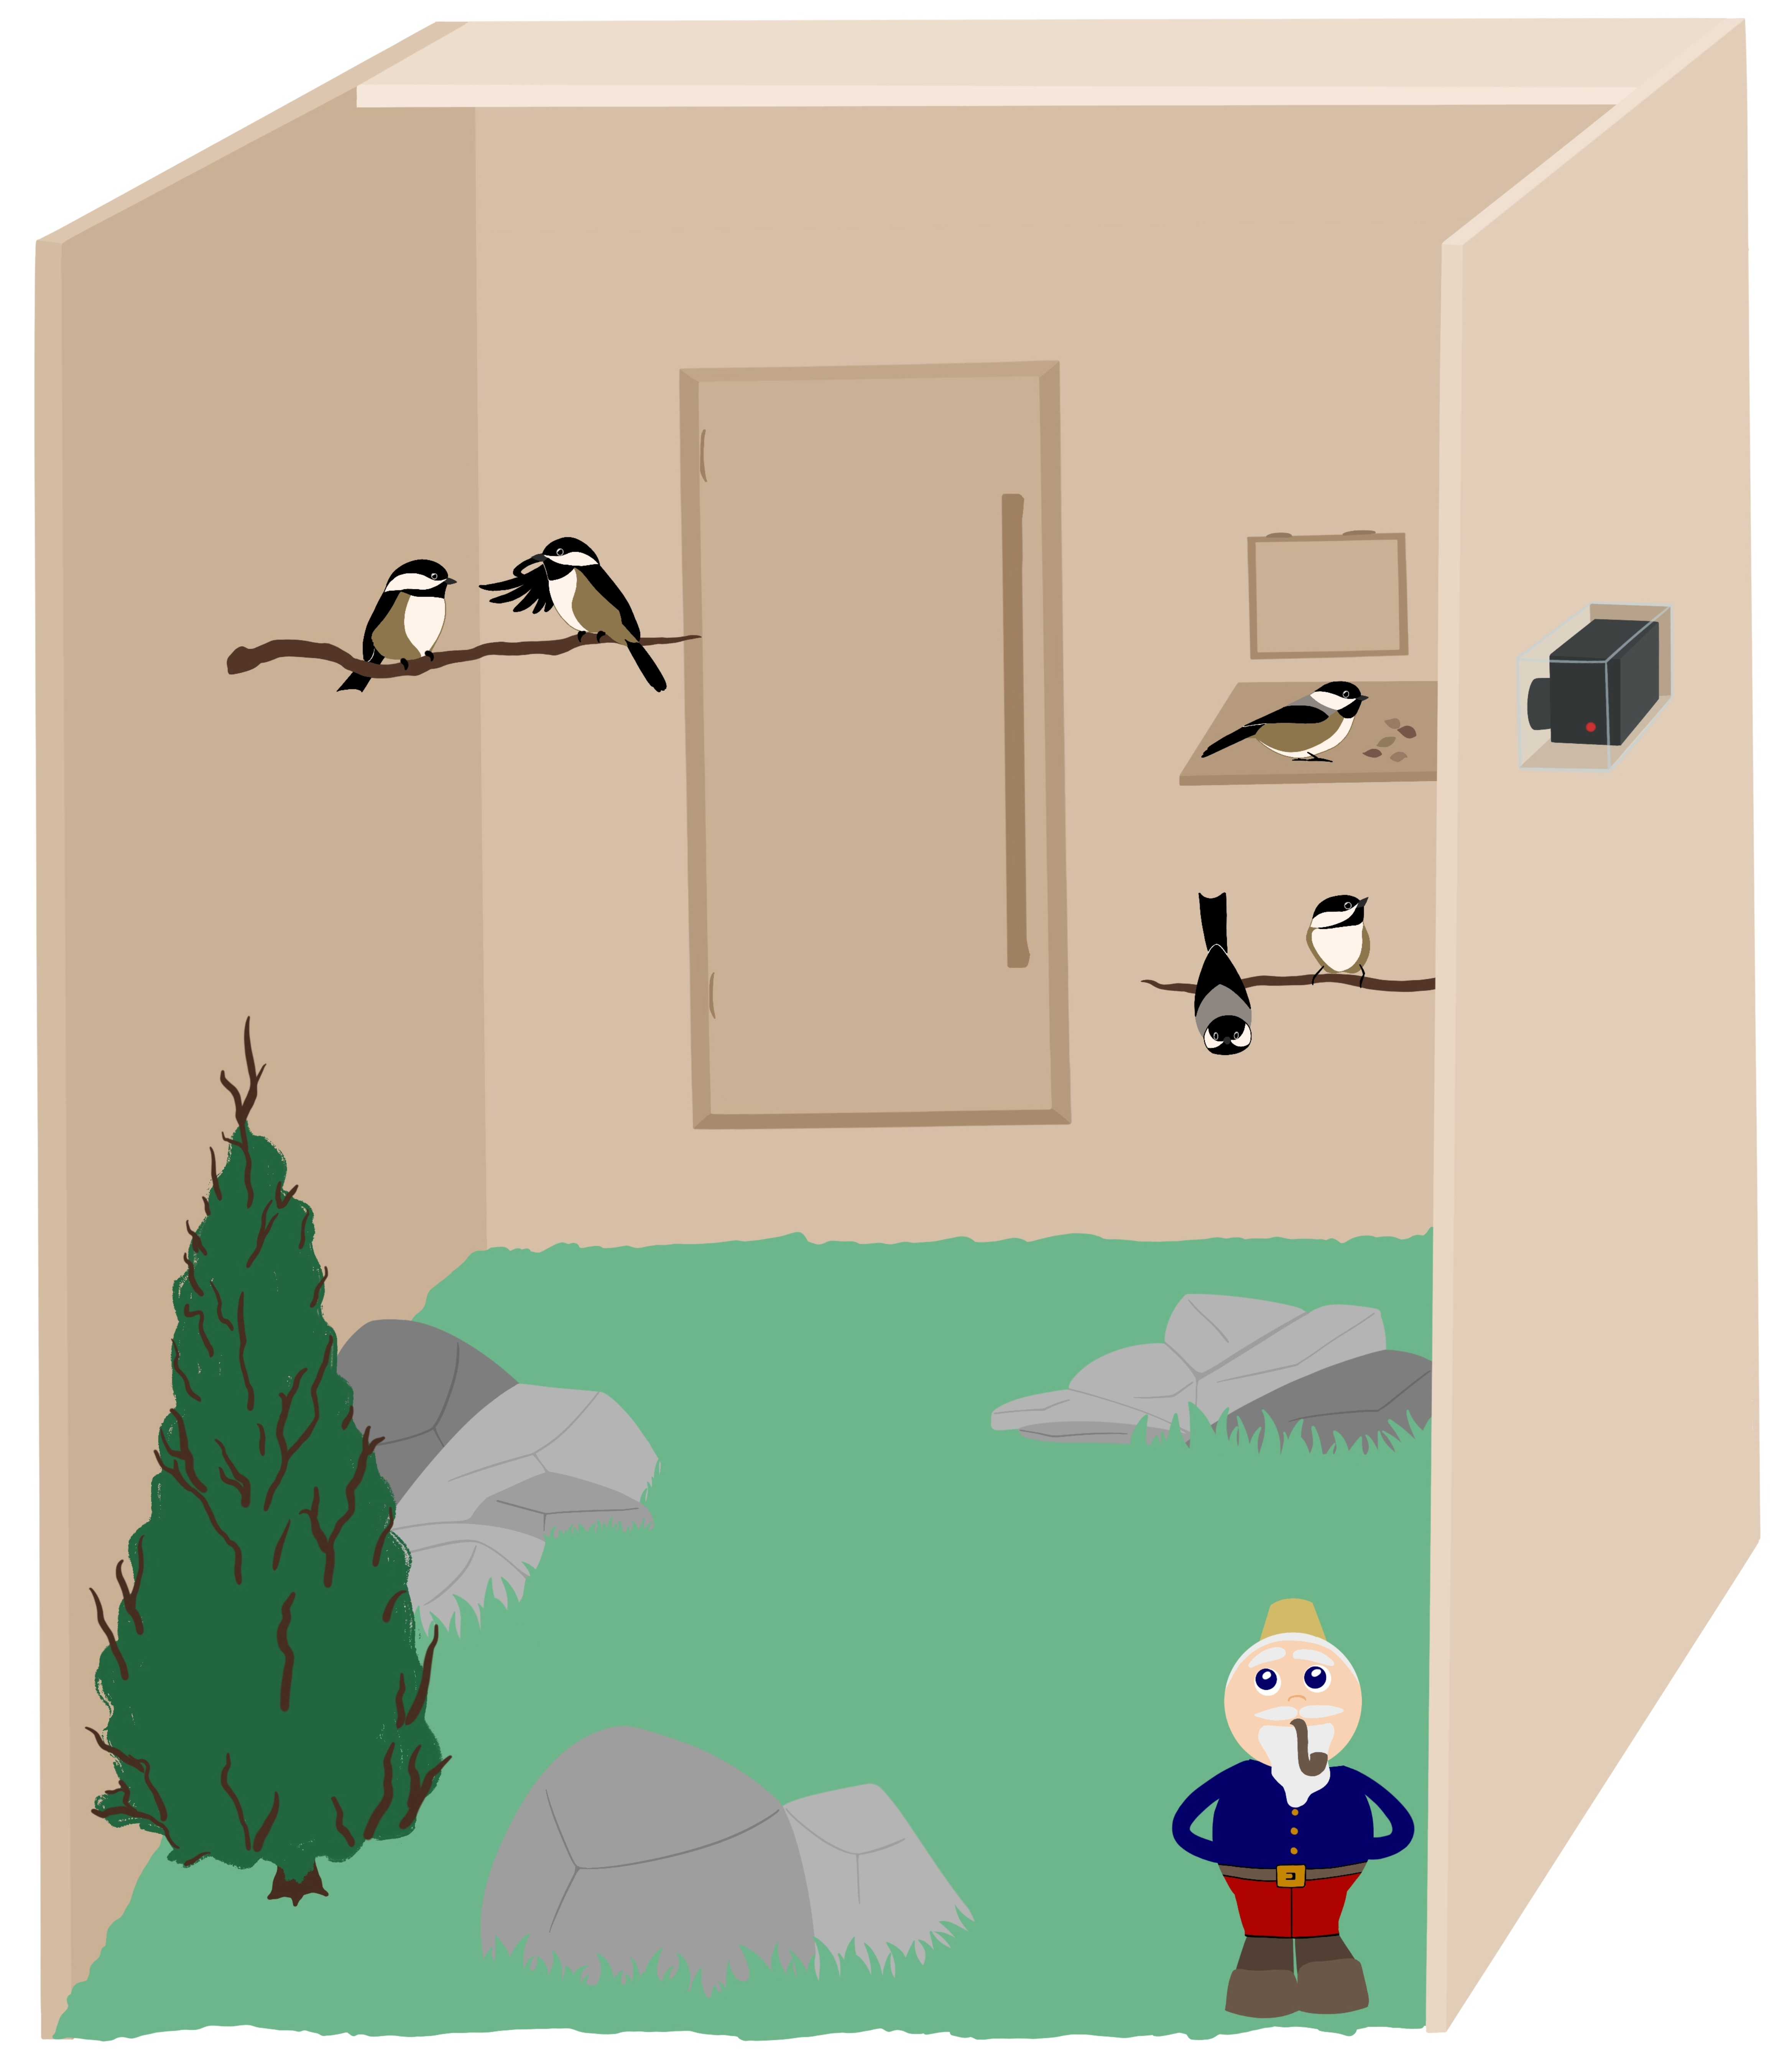
\includegraphics[width=0.7\textwidth]{/home/joshk/git_repositories/Phd_Thesis/Chapters/Ch4/Figures/Figure_1.jpg}
    \caption[\hspace{0.5cm}Depiction of experimental stress exposure (novel object) and infrared thermographic imaging in a selected flight enclosure.]{Depiction of experimental stress exposure (novel object) and infrared thermographic imaging in a selected flight enclosure. Black-capped chickadees (n = 5) within a given flight enclosure were simultaneously exposed to each individual stressor (here, the presence of a garden gnome), while individuals at raised feeding platforms were passively imaged with a remotely activated infrared thermographic camera.
}
\label{Fig4.1}
\end{figure}

\clearpage

\begin{figure}[ht]
	\centering
    \captionsetup{width=0.9\linewidth}
	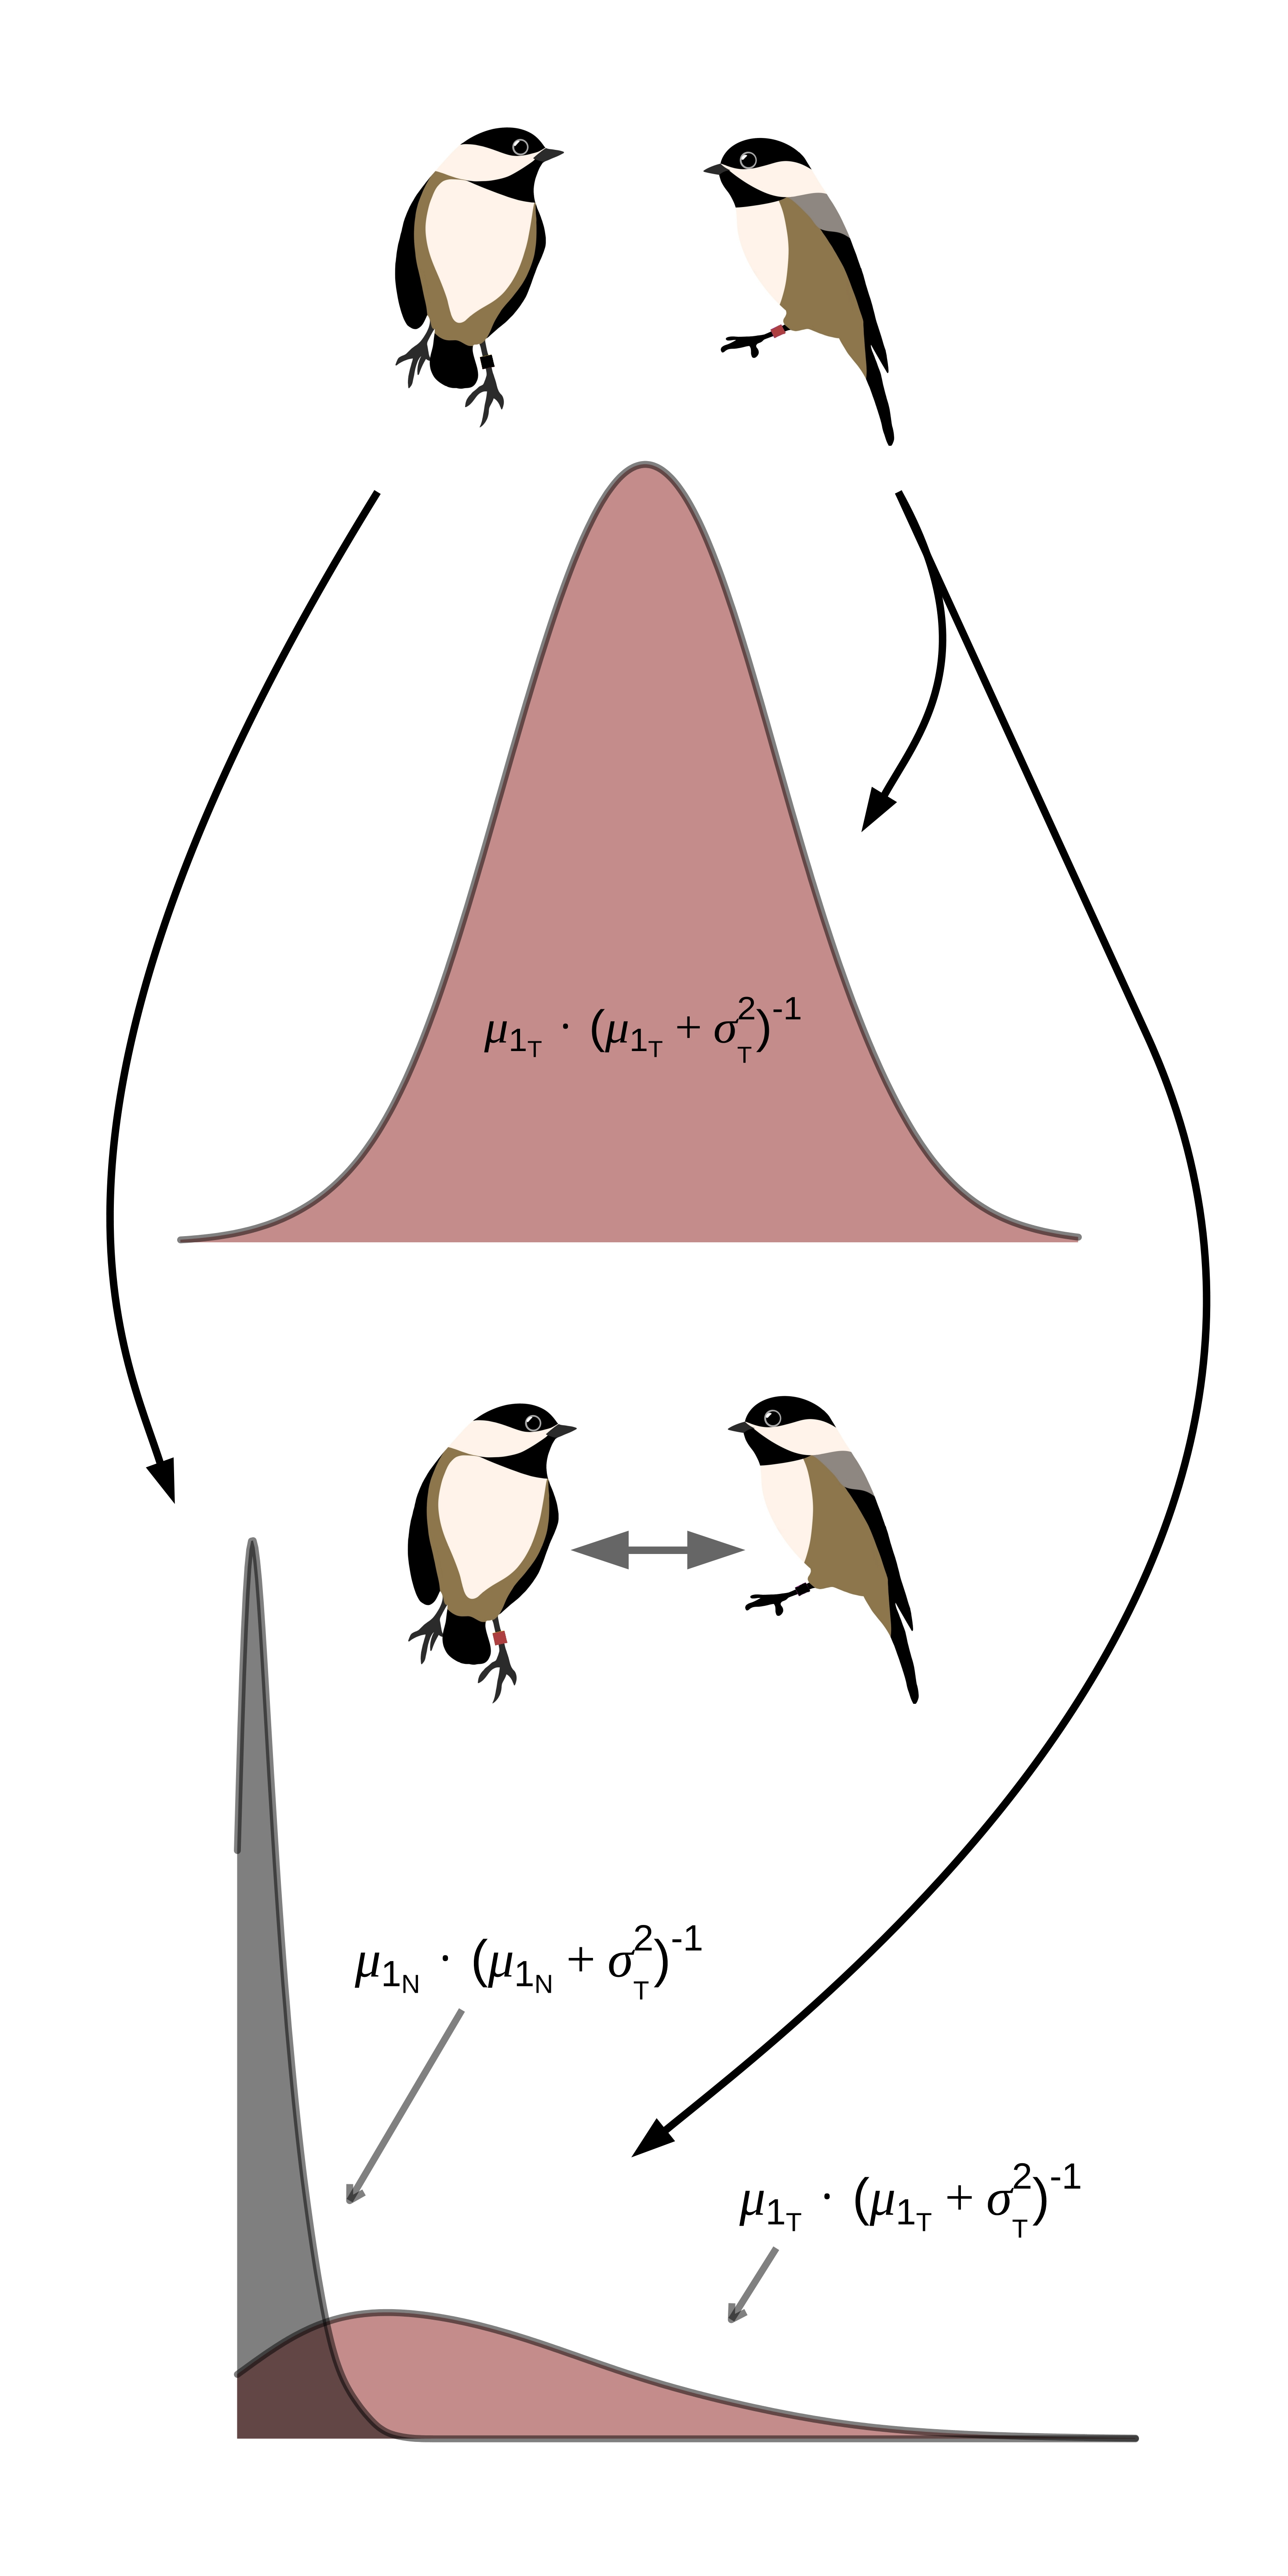
\includegraphics[width=0.5\textwidth]{/home/joshk/git_repositories/Phd_Thesis/Chapters/Ch4/Figures/Figure_2.jpg}
    \caption[\hspace{0.5cm}Method used to test for repeatability of stress-induced thermal responses among black-capped chickadees, while controlling for possible biases in the experimental process.]{Method used to test for repeatability of stress-induced thermal responses among black-capped chickadees, while controlling for possible biases in the experimental process. Repeatability values were calculated from a true model (maroon; subscripted "T") using methods described by Araya-Ajoy et al (2015). Individual identities were then scrambled to produce a null model (grey; subscripted "N"), from which repeatability values were again calculated as described above. Final repeatability estimates from true and null models were compared statistically.
    }
\label{Fig4.2}
\end{figure}
\clearpage

\begin{figure}[ht]
	\centering
	\includegraphics[width=\textwidth]{/home/joshk/git_repositories/Phd_Thesis/Chapters/Ch4/Figures/Figure_3Adj.jpg}
    \captionsetup{labelformat=empty}
    \caption[\hspace{0.5cm}Acute changes in eye region temperature (T\textsubscript{s}) and dry heat transfer (q\textsubscript{Tot}) following stress exposure in black-capped chickadee (n = 19) across ambient temperature.]{ }
\label{Fig4.3}
\end{figure}
\clearpage

\vspace{\baselineskip}
\vspace{\baselineskip}

\noindent\makebox[\textwidth][c]{
    \noindent\begin{minipage}[ht]{0.8\textwidth}
    \small
    \singlespacing
 
\noindent FIGURE 3 \hspace{0.5cm}Acute changes in eye region temperature (T\textsubscript{s}) and dry heat transfer (q\textsubscript{Tot}) following stress exposure in black-capped chickadee (n = 19) across ambient temperature. A | Average change in T\textsubscript{s} following stress exposure across ambient temperature ($^{\circ}$C) and time since exposure (s). Averages are derived from a Bayesian generalised additive mixed effects model (GAMM) and are marginalised across all other model predictors. T\textsubscript{s} decreases after stress exposure at ambient temperatures below thermoneutrality, and increases after stress exposure at ambient temperatures above thermoneutrality. B | Changes in q\textsubscript{Tot} of black-capped chickadees across both control and stress-exposed treatments, where slopes per treatment are permitted to vary among individuals. Each line represents the trend for a given individual at temperatures below, within, and above the thermoneutral zone (TNZ; estimated from Grossman and West, 1977), as predicted from a Bayesian GAMM. Dots represent averages per individual across 3 minutes of observation. Both trend lines and dots represent averages for each ambient temperature grouping (< TNZ, TNZ, > TNZ). Grey rectangles in panels A and B represent time when stress exposure treatments were applied in stress-exposed treatment groups. T\textsubscript{s} and q\textsubscript{Tot} were estimated by infra-red thermography (n = 5832 images) across 60 days.
\end{minipage}
}

\clearpage

% \begin{figure}[ht]
% 	\centering
% 	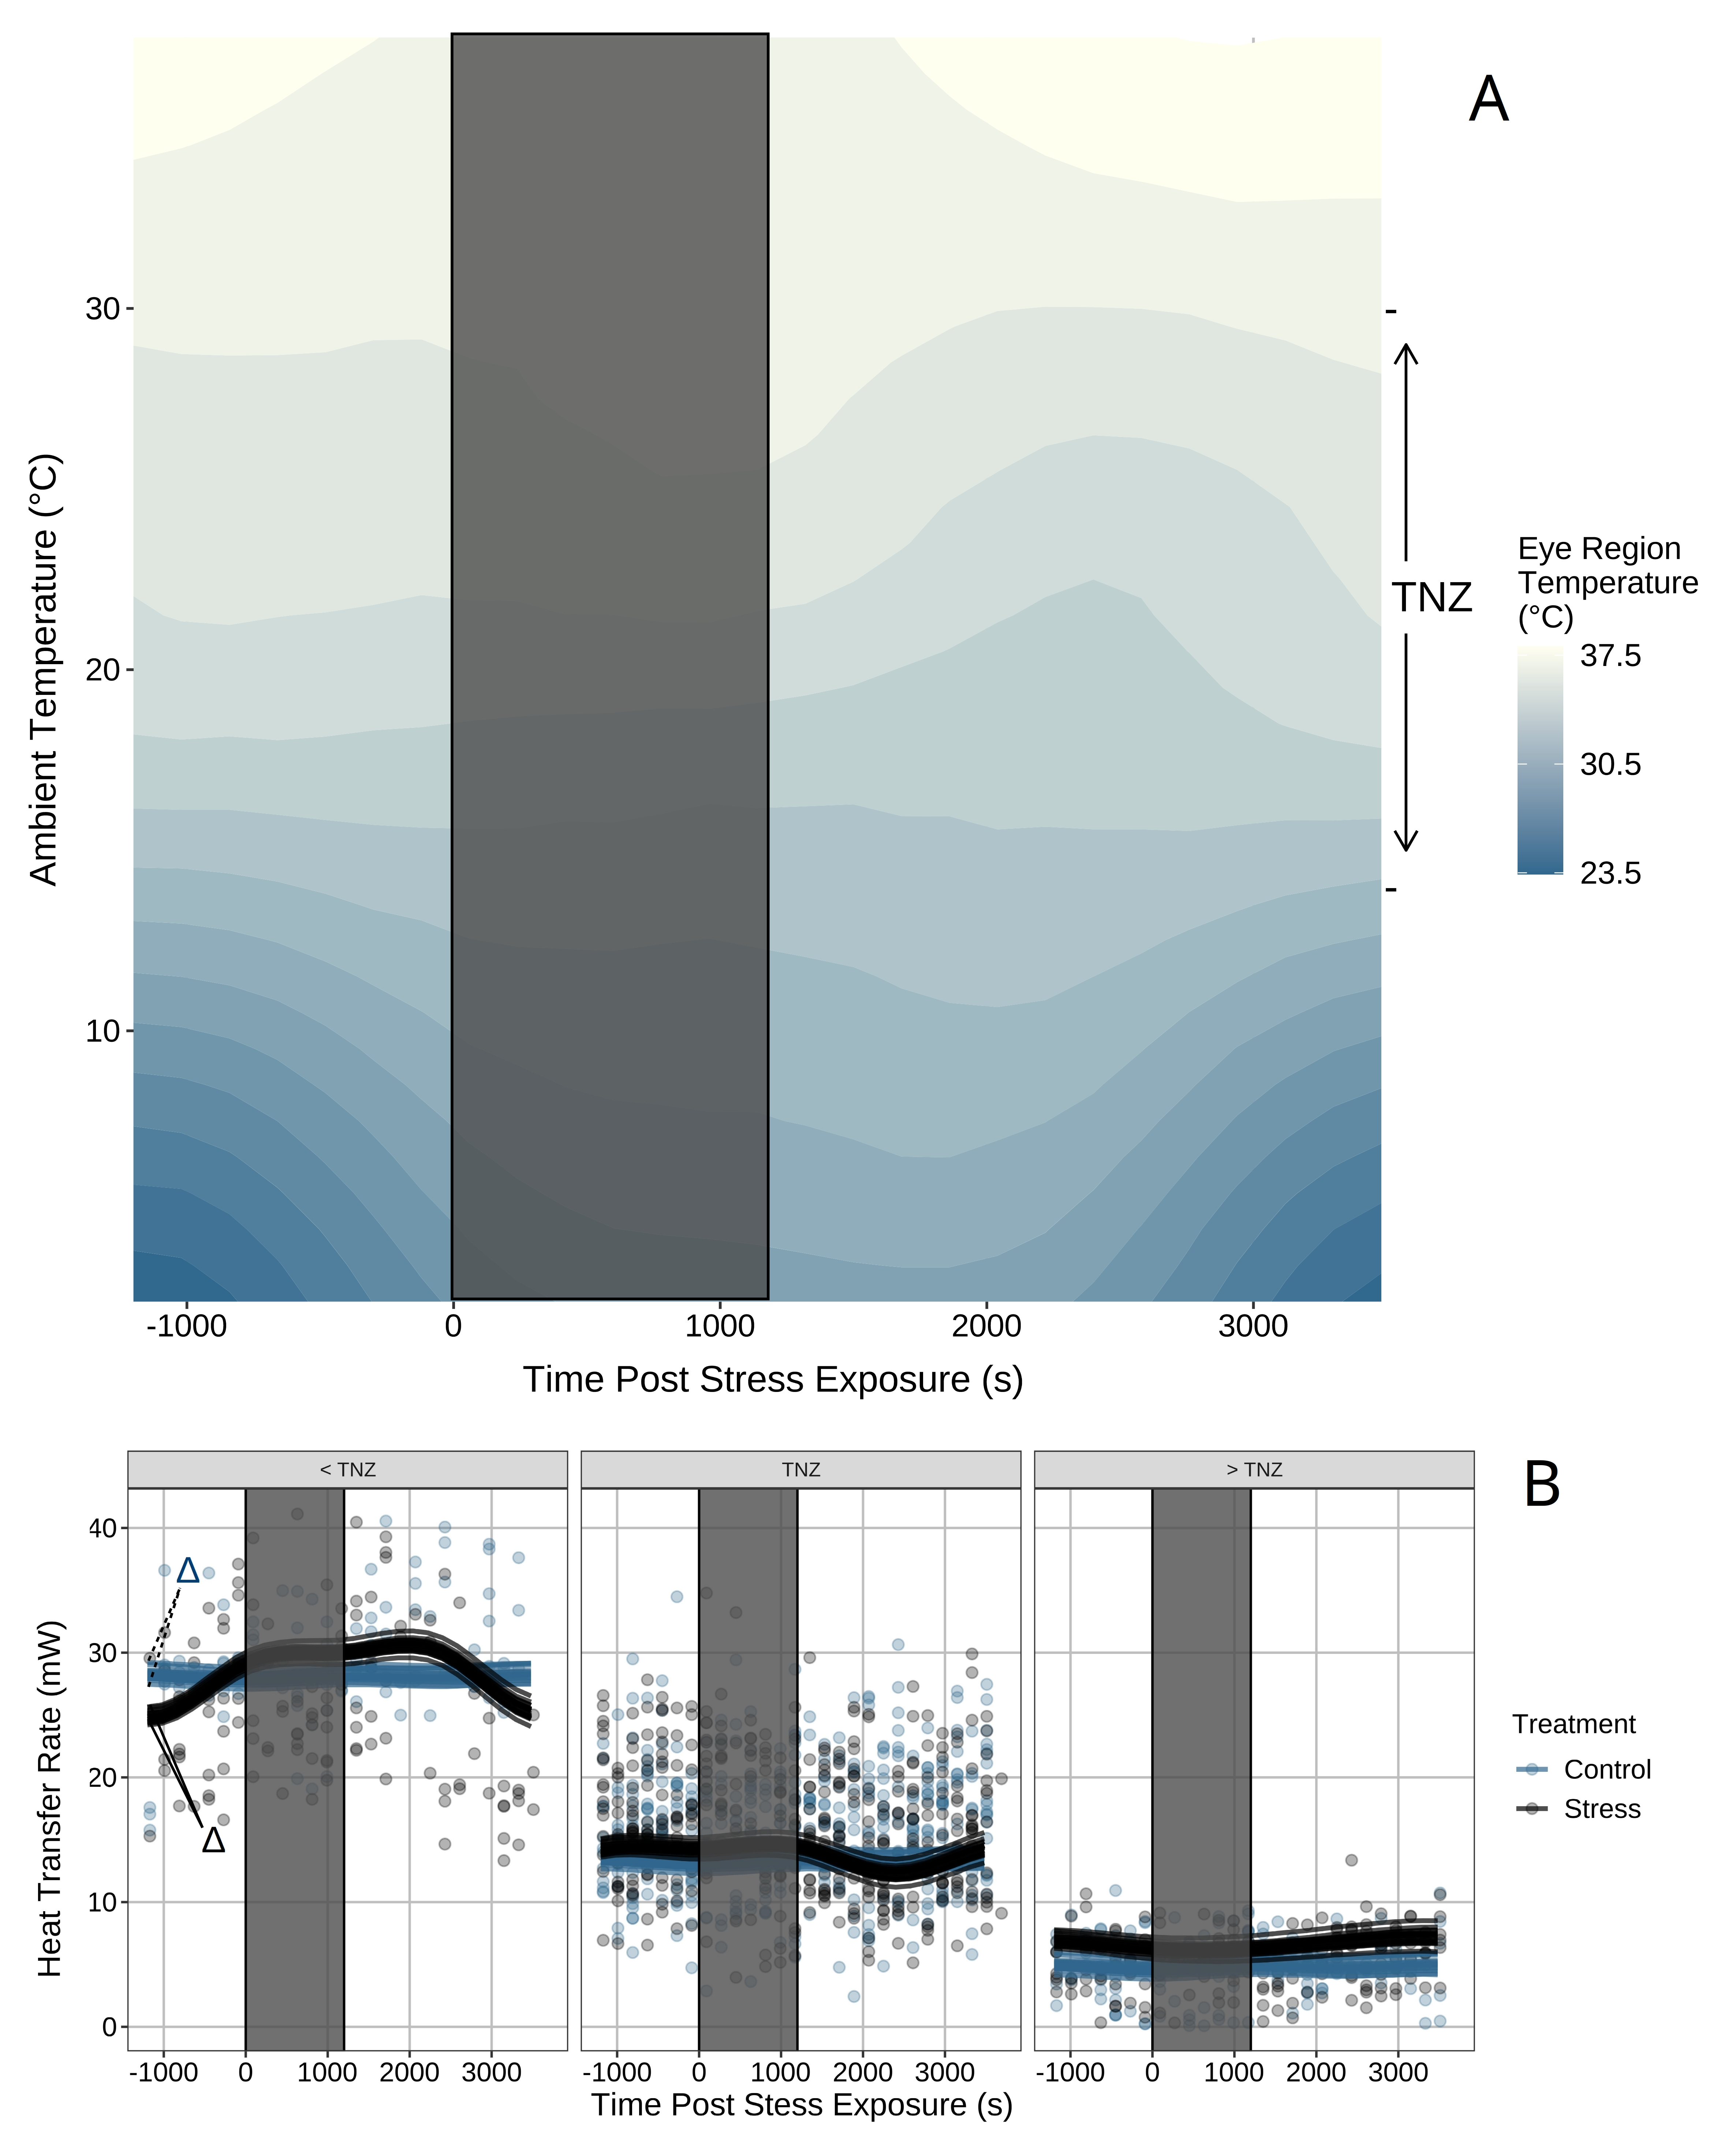
\includegraphics[width=0.65\textwidth]{/home/joshk/git_repositories/Phd_Thesis/Chapters/Ch4/Figures/Figure_3.jpg}
%     \caption[\textbf{Acute changes in eye region temperature (T\textsubscript{s}) and dry heat transfer (q\textsubscript{Tot}) following stress exposure in black-capped chickadee (n = 19) across ambient temperature.}]{\textbf{Acute changes in eye region temperature (T\textsubscript{s}) and dry heat transfer (q\textsubscript{Tot}) following stress exposure in black-capped chickadee (n = 19) across ambient temperature.} \textbf{A |} Average change in T\textsubscript{s} following stress exposure across ambient temperature ($^{\circ}$C) and time since exposure (s). Averages are derived from a Bayesian generalised additive mixed effects model (GAMM) and are marginalised across all other model predictors. \textbf{B |} Changes in q\textsubscript{Tot} of black-capped chickadees across both control and stress-exposed treatments, where slopes per treatment are permitted to vary among individuals. Each line represents the trend for a given individual at temperatures below, within, and above the thermoneutral zone (TNZ; estimated from Grossman and West, 1977), as predicted from a Bayesian GAMM. Dots represent averages per individual across 3 minutes of observation. Both trend lines and dots represent averages for each ambient temperature grouping (< TNZ, TNZ, > TNZ). Grey rectangles in panels A and B represent time when stress exposure treatments were applied in stress-exposed treatment groups. T\textsubscript{s} and q\textsubscript{Tot} were estimated by infra-red thermography (n = 5832 images) across 60 days.
% }
%     \label{F3}
% \end{figure}
% \clearpage 

\begin{figure}[ht]
	\centering
    \captionsetup{width=0.85\linewidth}
	\includegraphics[width=0.85\textwidth]{/home/joshk/git_repositories/Phd_Thesis/Chapters/Ch4/Figures/Figure_4_New.jpg}
    \caption[\hspace{0.5cm}Chronic changes in dry heat transfer (q\textsubscript{Tot}) at the eye region of black-capped chickadees (n = 19) following stress exposure across varying ambient temperatures.]{Chronic changes in dry heat transfer (q\textsubscript{Tot}) at the eye region of black-capped chickadees (n = 19) following stress exposure across varying ambient temperatures. Individual lines represents the predicted correlation between ambient temperature (here, mean-centered) and q\textsubscript{Tot} of individual black-capped chickadees during stress-exposure or control treatments. Bold black lines (solid and dashed) and accompanying delta ($\delta$) symbols indicate the spread of correlations between ambient temperature and q\textsubscript{Tot} across individuals, in control and stress exposure treatments respectively. Grey rectangle represents the thermoneutral zone (TNZ) for black-capped chickadees (estimated from Grossman and West, 1977). Correlations are estimated from a Bayesian generalised additive mixed effects model (GAMM) and marginalised across all environmental and experimental parameters. q\textsubscript{Tot} values were estimated by infra-red thermography (n = 5832 images) across 60 days. 
}
\label{Fig4.4}
\end{figure}
\clearpage 

\begin{figure}[ht]
	\centering
	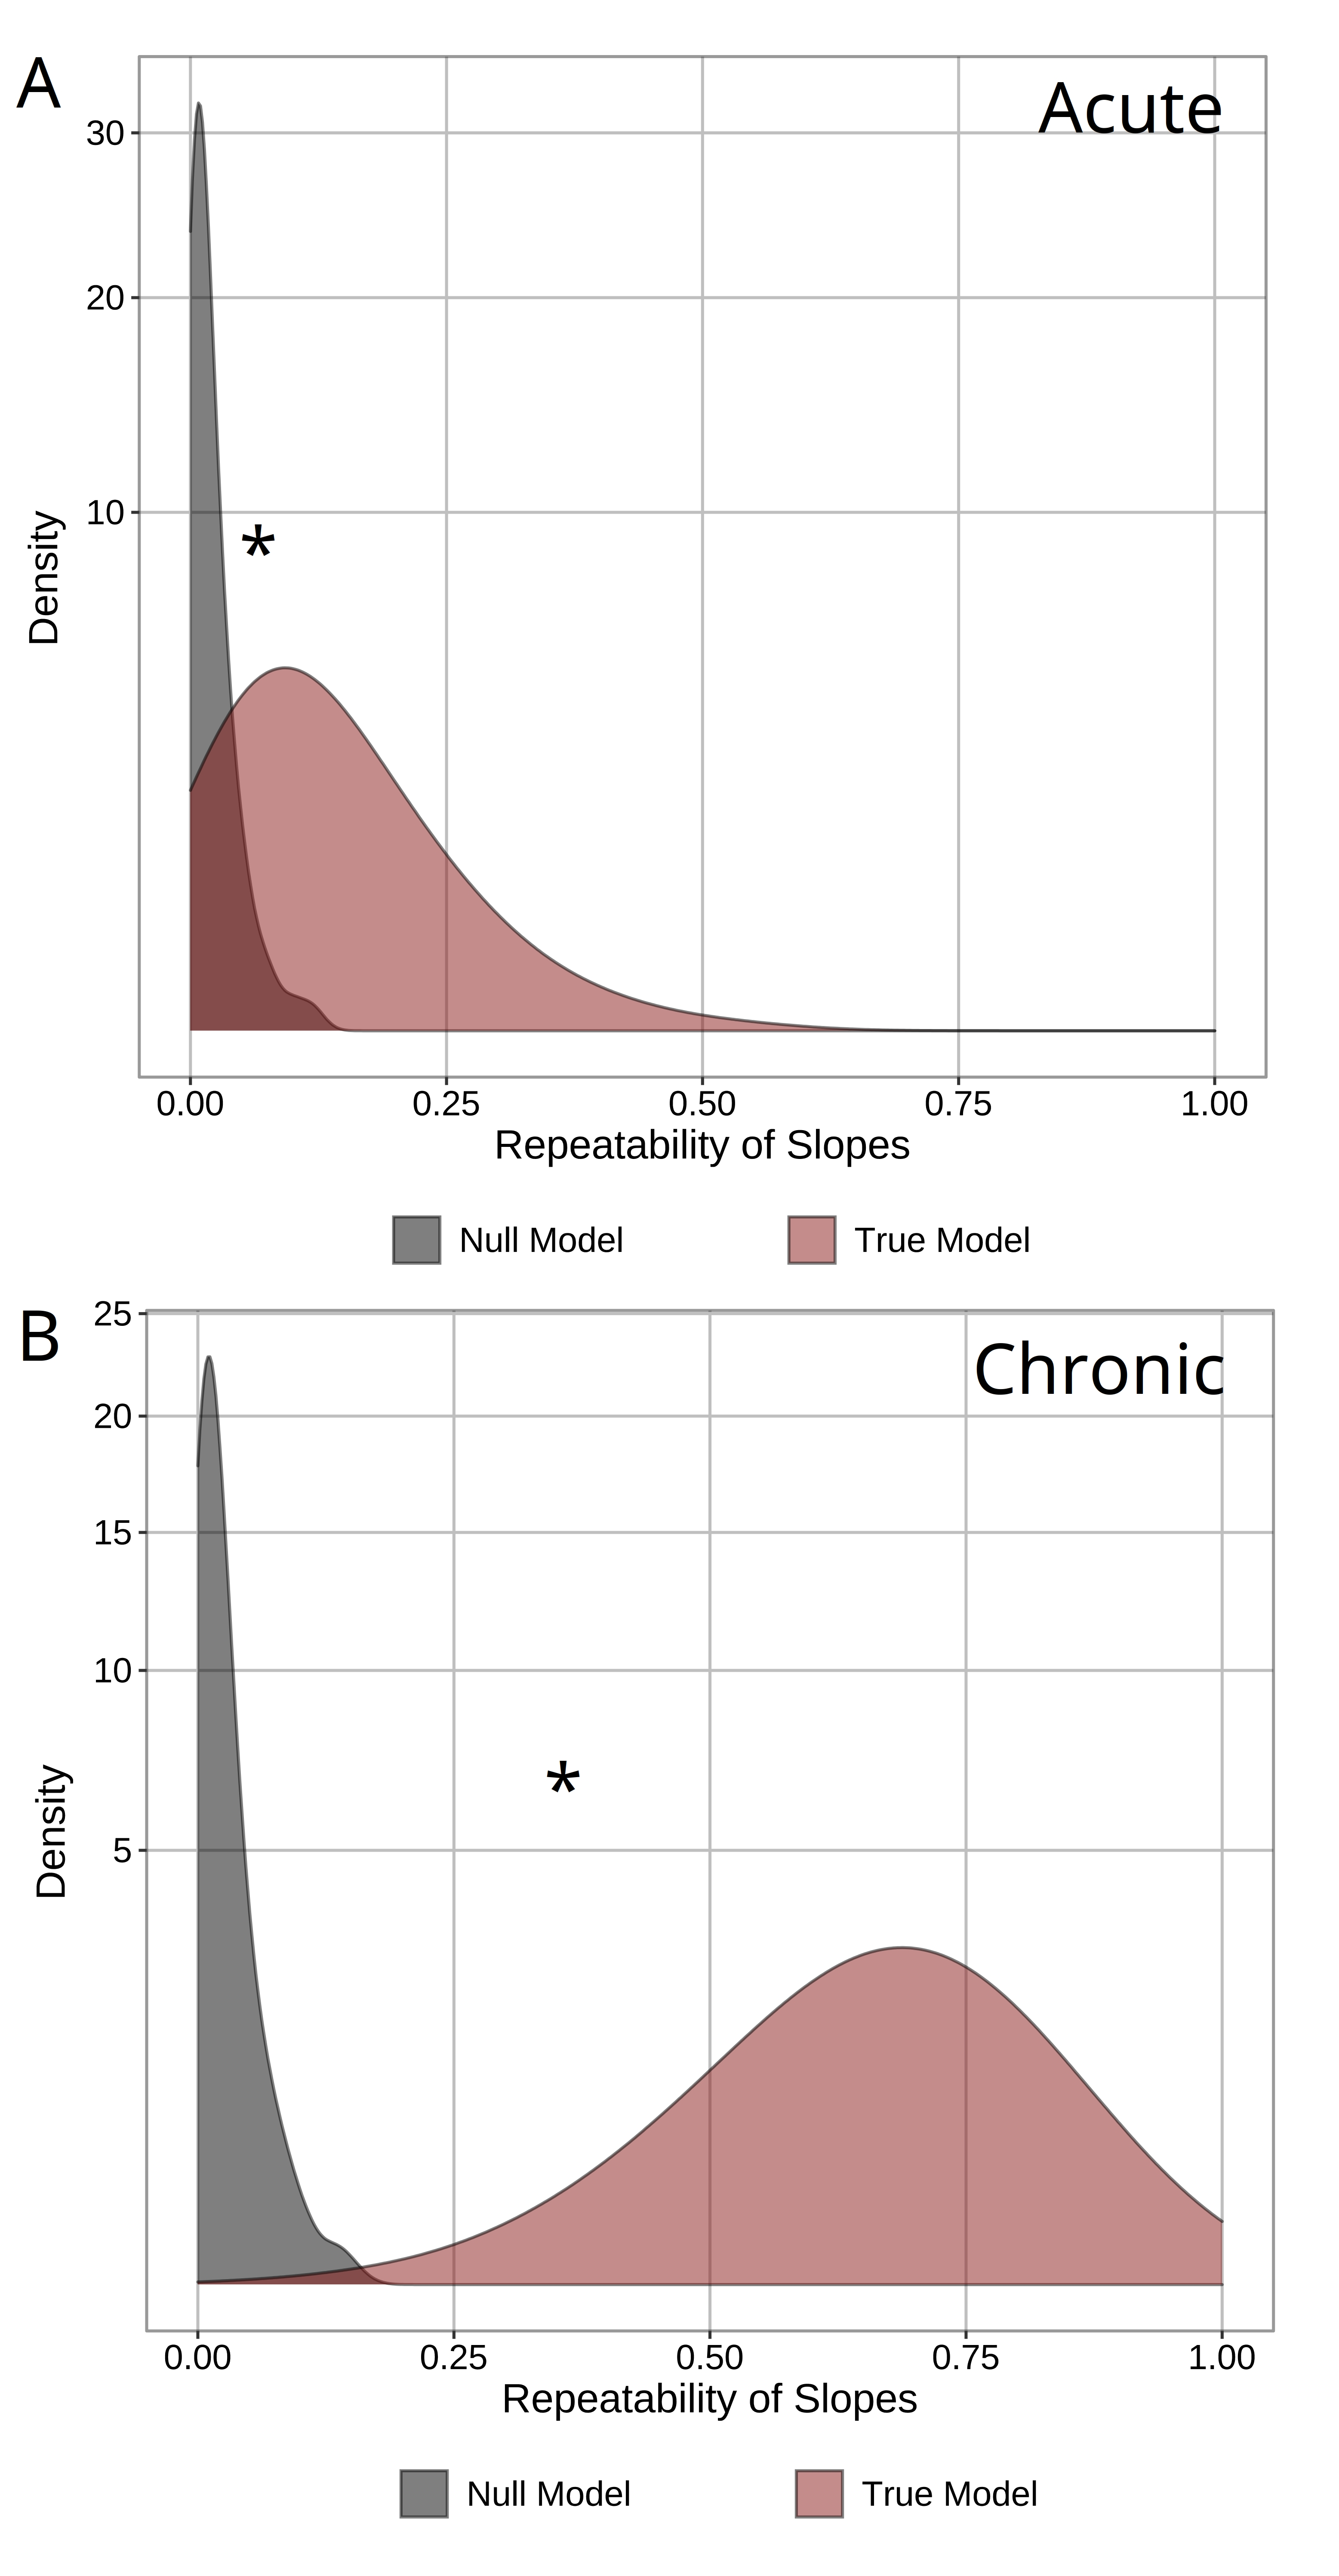
\includegraphics[width=.75\textwidth]{/home/joshk/git_repositories/Phd_Thesis/Chapters/Ch4/Figures/Figure_5.jpg}
    \captionsetup{labelformat=empty}
    \caption[\hspace{0.5cm}Repeatability of acute and chronic changes in dry heat transfer (q\textsubscript{Tot}) at the eye region during stress exposure in black-capped chickadees (n = 19).]{ }
\label{Fig4.5}
\end{figure}
\clearpage

\vspace{\baselineskip}
\vspace{\baselineskip}

\noindent\makebox[\textwidth][c]{
    \noindent\begin{minipage}[ht]{0.8\textwidth}
    \small
    \singlespacing
 
\noindent FIGURE 5 \hspace{0.5cm}Repeatability of acute and chronic changes in dry heat transfer (q\textsubscript{Tot}) at the eye region during stress exposure in black-capped chickadees (n = 19). Panels A and B represent distribution of repeatability values for acute and chronic responses to stress exposure, respectively. True model distributions (red) represent those of drawn from models where identity of individuals was correctly identified. In contrast, null model distributions (grey) represent those drawn from models where identity of individuals was randomly scrambled. A positive difference between true and null distributions (indicated by an asterisk, "*") implies that repeatability values from true models cannot be explained by biases in experimental methods (captured in null models) and are considered significant. Distributions are estimated from posteriors of Bayesian generalised additive mixed effects models (GAMM). Thermal responses to stress exposure represent those observed at the eye region of chickadees, using infra-red thermography across 60 days of observation.
\end{minipage}
}
\clearpage

\begin{figure}[ht]
	\centering
	\includegraphics[width=.75\textwidth]{/home/joshk/git_repositories/Phd_Thesis/Chapters/Ch4/Figures/Figure_6_New.jpg}
    \captionsetup{labelformat=empty}
    \caption[\hspace{0.5cm}Average effect of stress exposure on dry heat transfer (q\textsubscript{Tot}; reaction norm slopes) at the eye region of black-capped chickadees (n = 19) captured from urban and rural ecotypes (n = 9 urban, n = 10 rural).]{ }
\label{Fig4.6}
\end{figure}
\clearpage

\vspace{\baselineskip}
\vspace{\baselineskip}

\noindent\makebox[\textwidth][c]{
    \noindent\begin{minipage}[ht]{0.8\textwidth}
    \small
    \singlespacing
 
\noindent FIGURE 6 \hspace{0.5cm}Average effect of stress exposure on dry heat transfer (q\textsubscript{Tot}; reaction norm slopes) at the eye region of black-capped chickadees (n = 19) captured from urban and rural ecotypes (n = 9 urban, n = 10 rural). A | Average slopes of acute reaction norm across individuals captured at each ecotype. Reaction norm slopes represent the slopes of the linear interaction between treatment type and time post stress exposure (s) per individual. B | Average slopes of chronic reaction norms across individuals captured from each ecotype. Here, reaction norm slopes represent those of linear interactions between treatment type and ambient temperature ($^{\circ}$C) per individual. Error bars represent 95\% credible intervals around mean estimates. All reaction norm slopes were derived from Bayesian generalised additive mixed effects models (GAMMs).
\end{minipage}
}

\bibliography{/home/joshk/git_repositories/Phd_Thesis/Sorted_Thesis_Refs}
\bibliographystyle{besjournals}

\end{document}